\documentclass[10pt,twocolumn]{article}
\usepackage[margin=0.57in]{geometry}
\usepackage{array,amsmath,amssymb,booktabs,graphicx,xcolor,microtype,pifont,dsfont}
\usepackage{tabularx,multirow}
\usepackage[most]{tcolorbox}
\usepackage{tikz}
\usetikzlibrary{arrows.meta,positioning,fit,calc,shadows.blur,backgrounds}
\usepackage[font=small,labelfont=bf,skip=3pt]{caption}
\usepackage{titlesec}
\usepackage[hidelinks]{hyperref}
\titlespacing*{\section}{0pt}{6pt}{3pt}
\titlespacing*{\subsection}{0pt}{4pt}{2pt}
\setlength{\parskip}{1pt}
\definecolor{rel}{HTML}{2BB3C0}   % relation cyan (film palette)
\definecolor{ink}{HTML}{3A3F47}   % graphite
\definecolor{amber}{HTML}{F2A33A}
\definecolor{violet}{HTML}{8C7CF0}
\newcommand{\pt}[1]{\textcolor{rel}{\ding{\numexpr181+#1\relax}}}
\newcommand{\hl}[1]{\textcolor{rel!70!black}{\textbf{#1}}}
\newcommand{\code}[1]{\texttt{\small #1}}
\newcommand{\dn}[1]{\textsc{d-#1}}
\newcommand{\Y}{\textbf{\textcolor{rel!60!black}{Y}}}
\newcommand{\N}{\textcolor{gray}{--}}
\newcommand{\zcell}[1]{{\color{rel!#1!white}\rule{1.6mm}{1.6mm}}\hspace{0.2mm}}
% generated by make_figures.py table_relations from the registries; do not edit
\newcommand{\relsummary}{%
\begin{table}[t]
\centering\scriptsize
\setlength{\tabcolsep}{4pt}
\begin{tabular}{@{}lrrrrr@{}}
\toprule
Family & Impl. & Data gen & Attn & Readout & Planned \\
\midrule
structure & 9 & 0 & 7 & 0 & 4\\
geometry & 5 & 5 & 5 & 4 & 3\\
kinematics/body & 8 & 0 & 8 & 0 & 1\\
interaction & 5 & 5 & 5 & 4 & 6\\
task/procedure & 15 & 1 & 15 & 1 & 3\\
locomotion & 2 & 2 & 1 & 2 & 0\\
UI & 5 & 5 & 5 & 1 & 0\\
time & 0 & 0 & 0 & 0 & 3\\
probe readouts & 26 & 0 & 0 & 26 & 0\\
prop./aff./lang. & 0 & 0 & 0 & 0 & 8\\
\midrule
\textbf{total} & \textbf{75} & \textbf{18} & \textbf{46} & \textbf{38} & \textbf{28}\\
\bottomrule
\end{tabular}
\par\smallskip{\scriptsize Generated by \texttt{make\_figures.py} from the registries at \texttt{c18101e8}.}
\caption{\textbf{Relation factors by family.} Counts are computed from the registry; a factor can count in several columns. Planned = declared in the registry or catalogued (waves W2, P), not implemented. The full per-factor table is Table~\ref{tab:relations}.}
\label{tab:relations-summary}
\end{table}
}
\newcommand{\relfull}{%
\begin{table*}[t]
\centering\fontsize{6.8}{7.7}\selectfont
\setlength{\tabcolsep}{2pt}
\begin{tabularx}{\textwidth}{@{}>{\raggedright\arraybackslash}X >{\raggedright\arraybackslash}p{0.54in} p{0.37in} >{\raggedright\arraybackslash}p{0.82in} >{\raggedright\arraybackslash}p{1.12in} c c >{\raggedright\arraybackslash}p{1.04in} >{\raggedright\arraybackslash}p{0.7in}@{}}
\toprule
Factor & Operator & Form & Source(s) & Data gen (parts / transforms) & Attn & Read & Nets & Data envs \\
\midrule
\multicolumn{9}{@{}l}{\textsc{structure / edges} \;(9 implemented)}\\
\texttt{edge.\allowbreak{}node\_\allowbreak{}in\_\allowbreak{}assembly} & edge & bias & given & \textcolor{gray}{N} & \textbf{Y} & \textcolor{gray}{N} & arm,\allowbreak dual,\allowbreak leg,\allowbreak hum & --\\
\texttt{edge.\allowbreak{}same\_\allowbreak{}assembly} & edge & bias & given & \textcolor{gray}{N} & \textbf{Y} & \textcolor{gray}{N} & leg,\allowbreak hum,\allowbreak psi0 & --\\
\texttt{edge.\allowbreak{}same\_\allowbreak{}node} & edge & bias & given & \textcolor{gray}{N} & \textbf{Y} & \textcolor{gray}{N} & arm,\allowbreak dual,\allowbreak leg,\allowbreak hum,\allowbreak psi0 & --\\
\texttt{id.\allowbreak{}same\_\allowbreak{}assembly} & same & aug & given & \textcolor{gray}{N} & \textbf{Y} & \textcolor{gray}{N} & arm,\allowbreak dual,\allowbreak leg,\allowbreak hum,\allowbreak psi0 & --\\
\texttt{id.\allowbreak{}same\_\allowbreak{}body} & same & aug & given & \textcolor{gray}{N} & \textbf{Y} & \textcolor{gray}{N} & arm,\allowbreak dual & --\\
\texttt{id.\allowbreak{}slot\_\allowbreak{}handle} & inert & embed & given & \textcolor{gray}{N} & \textcolor{gray}{N} & \textcolor{gray}{N} & arm,\allowbreak dual & --\\
\texttt{msg.\allowbreak{}incidence} & inert & message & given & \textcolor{gray}{N} & \textcolor{gray}{N} & \textcolor{gray}{N} & arm,\allowbreak dual & --\\
\texttt{route.\allowbreak{}assembly\_\allowbreak{}reads} & same & mask & given & \textcolor{gray}{N} & \textbf{Y} & \textcolor{gray}{N} & arm,\allowbreak dual,\allowbreak leg,\allowbreak hum,\allowbreak psi0 & --\\
\texttt{route.\allowbreak{}own\_\allowbreak{}assembly} & same & mask & given & \textcolor{gray}{N} & \textbf{Y} & \textcolor{gray}{N} & arm,\allowbreak dual,\allowbreak leg,\allowbreak hum,\allowbreak psi0 & --\\
\midrule
\multicolumn{9}{@{}l}{\textsc{geometry} \;(5 implemented)}\\
\texttt{geo.\allowbreak{}above} & order & bias & given, gt$^\dagger$ & \textbf{Y}: table\_objects & \textbf{Y} & \textcolor{gray}{N} & arm,\allowbreak dual,\allowbreak ptr & arm,\allowbreak dual\\
\texttt{geo.\allowbreak{}depth3d} & sqdiff+diff & aug & probe, given, gt$^\dagger$ & \textbf{Y}: camera\_depth & \textbf{Y} & \textbf{Y} & arm,\allowbreak dual & arm,\allowbreak dual\\
\texttt{geo.\allowbreak{}normal\_\allowbreak{}align} & align & aug & given, probe, gt$^\dagger$ & \textbf{Y}: contact\_normal & \textbf{Y} & \textbf{Y} & arm,\allowbreak dual & arm,\allowbreak dual,\allowbreak mj-leg,\allowbreak wp-leg,\allowbreak simple\\
\texttt{geo.\allowbreak{}orient} & rel\_rot & aug & given, probe, gt$^\dagger$ & \textbf{Y}: table\_objects & \textbf{Y} & \textbf{Y} & arm,\allowbreak dual & arm,\allowbreak dual\\
\texttt{geo.\allowbreak{}pos3d} & sqdiff+diff & aug & given, probe, gt$^\dagger$ & \textbf{Y}: table\_objects & \textbf{Y} & \textbf{Y} & arm,\allowbreak dual,\allowbreak ptr & arm,\allowbreak dual\\
\midrule
\multicolumn{9}{@{}l}{\textsc{kinematics / body} \;(8 implemented)}\\
\texttt{edge.\allowbreak{}\{foot\_\allowbreak{}of,\allowbreak\ limb\_\allowbreak{}adjacent,\allowbreak\ over\_\allowbreak{}cell\}} (3) & edge & bias & given & \textcolor{gray}{N} & \textbf{Y} & \textcolor{gray}{N} & leg,\allowbreak hum & --\\
\texttt{edge.\allowbreak{}\{kin\_\allowbreak{}child,\allowbreak\ mirror\}} (2) & edge & bias & given & \textcolor{gray}{N} & \textbf{Y} & \textcolor{gray}{N} & leg,\allowbreak hum,\allowbreak psi0 & --\\
\texttt{edge.\allowbreak{}kin\_\allowbreak{}parent} & edge & bias & given & \textcolor{gray}{N} & \textbf{Y} & \textcolor{gray}{N} & arm,\allowbreak dual,\allowbreak leg,\allowbreak hum,\allowbreak psi0 & --\\
\texttt{kin.\allowbreak{}ancestor} & ancestor & bias & given & \textcolor{gray}{N} & \textbf{Y} & \textcolor{gray}{N} & arm,\allowbreak dual,\allowbreak leg,\allowbreak hum,\allowbreak psi0 & --\\
\texttt{kin.\allowbreak{}sibling} & hop & bias & given & \textcolor{gray}{N} & \textbf{Y} & \textcolor{gray}{N} & arm,\allowbreak dual,\allowbreak leg,\allowbreak hum,\allowbreak psi0 & --\\
\midrule
\multicolumn{9}{@{}l}{\textsc{physical interaction} \;(5 implemented)}\\
\texttt{ix.\allowbreak{}contact} & bilinear & aug & probe, gt$^\dagger$ & \textbf{Y}: grasp\_target & \textbf{Y} & \textbf{Y} & arm,\allowbreak dual & arm,\allowbreak dual\\
\texttt{ix.\allowbreak{}force\_\allowbreak{}flow} & flow & bias & probe, gt$^\dagger$ & \textbf{Y}: stack & \textbf{Y} & \textcolor{gray}{N} & arm,\allowbreak dual & arm,\allowbreak dual\\
\texttt{ix.\allowbreak{}handover} & bilinear & aug & probe, gt$^\dagger$ & \textbf{Y}: grasp\_target & \textbf{Y} & \textbf{Y} & dual & arm,\allowbreak dual\\
\texttt{ix.\allowbreak{}held\_\allowbreak{}by} & bilinear & aug & probe, gt$^\dagger$ & \textbf{Y}: grasp\_target & \textbf{Y} & \textbf{Y} & arm,\allowbreak dual & arm,\allowbreak dual\\
\texttt{ix.\allowbreak{}support} & bilinear & aug & probe, gt$^\dagger$ & \textbf{Y}: stack & \textbf{Y} & \textbf{Y} & arm,\allowbreak dual & arm,\allowbreak dual\\
\midrule
\multicolumn{9}{@{}l}{\textsc{task / procedure} \;(15 implemented)}\\
\texttt{edge.\allowbreak{}\{actor\_\allowbreak{}of,\allowbreak\ consumed\_\allowbreak{}by,\allowbreak\ destination\_\allowbreak{}of,\allowbreak\ enables,\allowbreak\ maintained,\allowbreak\ node\_\allowbreak{}actor\_\allowbreak{}of,\allowbreak\ output\_\allowbreak{}to,\allowbreak\ patient\_\allowbreak{}of,\allowbreak\ pred\_\allowbreak{}arg,\allowbreak\ produced,\allowbreak\ role\_\allowbreak{}in\_\allowbreak{}event,\allowbreak\ role\_\allowbreak{}points\_\allowbreak{}to,\allowbreak\ support\_\allowbreak{}of,\allowbreak\ target\_\allowbreak{}of\}} (14) & edge & bias & given & \textcolor{gray}{N} & \textbf{Y} & \textcolor{gray}{N} & arm,\allowbreak dual & --\\
\texttt{task.\allowbreak{}next\_\allowbreak{}contact} & bilinear & aug & probe, gt$^\dagger$ & \textbf{Y}: \textit{reveal}, \textit{surprise} & \textbf{Y} & \textbf{Y} & arm,\allowbreak dual & arm,\allowbreak dual,\allowbreak mj-leg,\allowbreak wp-leg,\allowbreak simple\\
\midrule
\multicolumn{9}{@{}l}{\textsc{locomotion} \;(2 implemented)}\\
\texttt{leg.\allowbreak{}com\_\allowbreak{}support} & inert & readout & given & \textbf{Y}: terrain\_steps & \textcolor{gray}{N} & \textbf{Y} & leg,\allowbreak hum & mj-leg,\allowbreak wp-leg\\
\texttt{leg.\allowbreak{}foothold} & bilinear & aug & probe, gt$^\dagger$ & \textbf{Y}: terrain\_steps & \textbf{Y} & \textbf{Y} & leg,\allowbreak hum & mj-leg,\allowbreak wp-leg\\
\midrule
\multicolumn{9}{@{}l}{\textsc{UI} \;(5 implemented)}\\
\texttt{ui.\allowbreak{}above} & order & bias & given & \textbf{Y}: cw\_viewport, cw\_depth & \textbf{Y} & \textcolor{gray}{N} & ptr & cw\\
\texttt{ui.\allowbreak{}drag\_\allowbreak{}to} & bilinear & aug & probe, gt$^\dagger$ & \textbf{Y}: cw\_viewport, cw\_depth & \textbf{Y} & \textbf{Y} & ptr & none$^\ddagger$\\
\texttt{ui.\allowbreak{}focus\_\allowbreak{}next} & edge & bias & given, gt$^\dagger$ & \textbf{Y}: cw\_viewport, cw\_depth & \textbf{Y} & \textcolor{gray}{N} & ptr & cw\\
\texttt{ui.\allowbreak{}label\_\allowbreak{}for} & edge & bias & given, gt$^\dagger$ & \textbf{Y}: cw\_viewport, cw\_depth, \textit{reveal}, \textit{surprise} & \textbf{Y} & \textcolor{gray}{N} & ptr & cw\\
\texttt{ui.\allowbreak{}same\_\allowbreak{}window} & same & bias & given & \textbf{Y}: cw\_viewport, cw\_depth & \textbf{Y} & \textcolor{gray}{N} & ptr & cw\\
\midrule
\multicolumn{9}{@{}l}{\textsc{probe readouts} \;(26 implemented)}\\
\texttt{probe.\allowbreak{}arm.\allowbreak{}\{acting\_\allowbreak{}on,\allowbreak\ focused\_\allowbreak{}on,\allowbreak\ goal\_\allowbreak{}effect,\allowbreak\ held\_\allowbreak{}by,\allowbreak\ looking\_\allowbreak{}at,\allowbreak\ observed\_\allowbreak{}effect,\allowbreak\ rel\_\allowbreak{}pos,\allowbreak\ subtask,\allowbreak\ visible\}} (9) & inert & readout & given & \textcolor{gray}{N} & \textcolor{gray}{N} & \textbf{Y} & arm,\allowbreak dual & --\\
\texttt{probe.\allowbreak{}legged.\allowbreak{}\{contact,\allowbreak\ disp,\allowbreak\ fall,\allowbreak\ goal,\allowbreak\ subtask\}} (5) & inert & readout & given & \textcolor{gray}{N} & \textcolor{gray}{N} & \textbf{Y} & leg,\allowbreak hum & --\\
\texttt{probe.\allowbreak{}pointer.\allowbreak{}\{phase,\allowbreak\ rel,\allowbreak\ slot\}} (3) & inert & readout & given & \textcolor{gray}{N} & \textcolor{gray}{N} & \textbf{Y} & ptr & --\\
\texttt{probe.\allowbreak{}psi0.\allowbreak{}\{active\_\allowbreak{}hand,\allowbreak\ base\_\allowbreak{}cmd,\allowbreak\ base\_\allowbreak{}disp,\allowbreak\ contact,\allowbreak\ grasp\_\allowbreak{}face,\allowbreak\ grasp\_\allowbreak{}pt,\allowbreak\ hand\_\allowbreak{}dist,\allowbreak\ lift,\allowbreak\ target\_\allowbreak{}pos\}} (9) & inert & readout & given & \textcolor{gray}{N} & \textcolor{gray}{N} & \textbf{Y} & psi0 & --\\
\bottomrule
\end{tabularx}
\par\smallskip
{\scriptsize Generated by \texttt{make\_figures.py} from the registries at \texttt{c18101e8}.}
\caption{\textbf{Every implemented relation factor.} 75 factors: 18 generate or label data, 46 act on attention logits or masks, 38 supervise a readout (several per factor possible). Rows with identical classification are merged (\texttt{edge.*}, \texttt{probe.<net>.*}; count in parentheses). gt$^\dagger$ = gt (training only): simulator truth, never a deployable input. Data gen: a data generator is declared or a relgen label exists (scene parts upright, transforms italic); probe targets are task-pipeline packet labels, hence N. Attn: form $\in$ \{bias, aug, gate, mask\}. Read: a readout is declared. Nets: families whose \texttt{resolve(family=...)} accepts the factor. Data envs: label caps and scene part available; $^\ddagger$ no registered environment provides the caps yet. Fig.~\ref{fig:tiles} draws one tile per factor.}
\label{tab:relations}
\end{table*}
}
\newcommand{\relplanned}{%
\begin{table*}[t]
\centering\scriptsize
\setlength{\tabcolsep}{2.4pt}
\begin{tabularx}{\textwidth}{@{}>{\raggedright\arraybackslash}p{1.15in} p{0.88in} >{\raggedright\arraybackslash}p{1.3in} >{\raggedright\arraybackslash}p{0.8in} >{\raggedright\arraybackslash}X >{\raggedright\arraybackslash}p{0.7in}@{}}
\toprule
Intended entry & Status & Catalog family & Operator $\times$ form & Needs (label caps; scene part) & Envs \\
\midrule
\multicolumn{6}{@{}l}{\textsc{structure / edges} \;(4 planned)}\\
\texttt{id.\allowbreak{}same\_\allowbreak{}material} & planned (W2) & same-X & same $\times$ aug & \texttt{materials}; needs material ids & all\\
\textit{\texttt{id.\allowbreak{}same\_\allowbreak{}part\_\allowbreak{}class}} & planned (P) & symmetry / lattice; equivalence & same + edge & -- & simple, arm\\
\textit{\texttt{id.\allowbreak{}same\_\allowbreak{}segment}} & planned (P) & segmentation & same & needs image-patch tokens with masks & arm\\
\textit{\texttt{id.\allowbreak{}scene\_\allowbreak{}parent}} & planned (W2) & hierarchy & ancestor + hop & -- & arm, legged, simple\\
\midrule
\multicolumn{6}{@{}l}{\textsc{geometry} \;(3 planned)}\\
\textit{\texttt{geo.\allowbreak{}extent}} & planned (P) & shape and scale & unary + sim & \texttt{extent} & arm, dual\\
\textit{\texttt{geo.\allowbreak{}occludes}} & planned (P) & visibility & unary + edge & -- & arm, dual\\
\textit{\texttt{geo.\allowbreak{}surface\_\allowbreak{}normal}} & planned (W2) & surface directions & align $\times$ aug & \texttt{surface\_\allowbreak{}normal} & arm, dual\\
\midrule
\multicolumn{6}{@{}l}{\textsc{kinematics / body} \;(1 planned)}\\
\textit{\texttt{kin.\allowbreak{}cross\_\allowbreak{}morphology}} & planned (P) & mirror / morphology correspondence & same + edge & -- & simple\\
\midrule
\multicolumn{6}{@{}l}{\textsc{physical interaction} \;(6 planned)}\\
\texttt{ix.\allowbreak{}articulation} & planned (W2) & attachment / articulation & bilinear + align & \texttt{articulation\_\allowbreak{}pairs}; needs a \texttt{drawer} / \texttt{door} part & arm\\
\textit{\texttt{ix.\allowbreak{}collision\_\allowbreak{}seq}} & planned (W2) & collisions over time & flow & -- & arm, dual, legged\\
\texttt{ix.\allowbreak{}contains} & planned (W2) & region topology; containment of content & bilinear + edge & \texttt{contains\_\allowbreak{}pairs}; needs \texttt{bin} part; \texttt{bin} part & arm, dual, cw\\
\textit{\texttt{ix.\allowbreak{}impulse\_\allowbreak{}flow}} & planned (W2) & force transfer & flow $\times$ bias & \texttt{support\_\allowbreak{}pairs}, \texttt{contact\_\allowbreak{}forces} & arm, dual\\
\texttt{ix.\allowbreak{}mating} & planned (W2) & mating / insertion & bilinear + align & \texttt{mating\_\allowbreak{}pairs}; support\_insert task exists & arm\\
\texttt{ix.\allowbreak{}tool\_\allowbreak{}target} & planned (W2) & tool use & bilinear $\times$ gate & \texttt{tool\_\allowbreak{}pairs}; needs a tool part & arm\\
\midrule
\multicolumn{6}{@{}l}{\textsc{task / procedure} \;(3 planned)}\\
\texttt{rel.\allowbreak{}task\_\allowbreak{}relevance} & planned (W2) & relevance / salience & unary $\times$ gate, readout & -- & arm, dual, cw\\
\texttt{task.\allowbreak{}cause\_\allowbreak{}effect} & planned (W2) & causality & edge + flow & labels from task receipts + interventions & arm, dual\\
\texttt{task.\allowbreak{}precedes} & planned (W2) & prerequisites & ancestor & -- & arm, dual\\
\midrule
\multicolumn{6}{@{}l}{\textsc{time} \;(3 planned)}\\
\textit{\texttt{time.\allowbreak{}co\_\allowbreak{}motion}} & planned (P) & motion & sim + diff & velocity labels exist & arm, dual, legged\\
\texttt{time.\allowbreak{}phase\_\allowbreak{}sync} & planned (W2) & periodicity / phase & rel\_rot + align & legged gait legs & legged\\
\texttt{time.\allowbreak{}same\_\allowbreak{}track} & planned (registry) & correspondence (declared) & same $\times$ aug & -- & --\\
\midrule
\multicolumn{6}{@{}l}{\textsc{properties / affordance / language} \;(8 planned)}\\
\texttt{aff.\allowbreak{}\textless{}verb\textgreater{}} & planned (P) & affordance scores & unary $\times$ readout & labels need per-object scripted affordance tables & arm, dual\\
\textit{\texttt{aff.\allowbreak{}affords\_\allowbreak{}at}} & planned (W2) & affordance pairs & bilinear $\times$ gate & -- & arm, cw\\
\textit{\texttt{aff.\allowbreak{}compatible}} & planned (P) & compatibility & bilinear + sim $\times$ gate & -- & --\\
\textit{\texttt{aff.\allowbreak{}safe\_\allowbreak{}region}} & planned (P) & safety regions & unary & -- & arm\\
\texttt{lang.\allowbreak{}refers\_\allowbreak{}to} & planned (W2) & text grounding & bilinear & needs instruction tokens in the arm ctx & --\\
\textit{\texttt{lang.\allowbreak{}sim}} & planned (P) & semantic similarity & sim & -- & --\\
\texttt{prop.\allowbreak{}*} & planned (P) & physical properties & unary + sim & \texttt{inertia}, \texttt{materials}; labels exist in MuJoCo: \texttt{inertia}, \texttt{materials} & arm, dual\\
\texttt{prop.\allowbreak{}vel} & planned (P) & fields and flows & unary & -- & --\\
\midrule
\multicolumn{6}{@{}p{\dimexpr\textwidth-4.8pt\relax}}{\textsc{out of scope} (3 families; no physics or sensing for them in our environments): fields and flows; fluids, thermal, electrical, magnetic, optical, chemical; mechanics.}\\
\bottomrule
\end{tabularx}
\par\smallskip
{\scriptsize Generated by \texttt{make\_figures.py} from \texttt{research/relations\_catalog.md} and the registries at \texttt{c18101e8}.}
\caption{\textbf{Planned and out-of-scope relations.} 28 planned entries (1 declared in the registry with status planned, 27 from the candidate catalog, waves W2 and P); 3 out-of-scope families. Italic names are proposed (the catalog names no entry). None is implemented, so no result in this paper depends on them. Meta properties of relations (catalog section K and 3 rows tagged M, e.g.\ joint states, costs) are not factors and are excluded; 4 epistemic mechanisms (confidence scaling, soft edges, the reveal / surprise / noise / occlude transforms) are implemented but are not attention factors.}
\label{tab:relations-planned}
\end{table*}
}

% generated by make_figures.py embodiments from the artifact stores; do not edit
\newcommand{\embtotal}{251}
\newcommand{\embtrained}{150}
\newcommand{\embarms}{150}
\newcommand{\embarmproc}{108}
\newcommand{\embdual}{19}
\newcommand{\emblegged}{80}
\newcommand{\embphum}{64}
\newcommand{\embtable}{%
\par\medskip\noindent\begin{minipage}{\columnwidth}\centering\scriptsize\setlength{\tabcolsep}{2.5pt}
\begin{tabularx}{\columnwidth}{@{}>{\raggedright\arraybackslash}X r r >{\raggedright\arraybackslash}p{0.95in}@{}}
\toprule
Embodiment class & Sim. & Trained & Evidence \\
\midrule
single arms: menagerie + fixture arms, each with each gripper module (pg2, tf3) & 42 & 17 & teacher validation (20 seeds) + armdiv admission screens\\
procedural arms \texttt{arm\_gen\_v2} (\texttt{pa2s<seed>}, train and sealed seeds) $\times$ gripper & 108 & 48 & armdiv admission screens (built keys only)\\
dual-arm rigs (unordered arm pairs) + ALOHA & 19 & 6 & dual teacher validation, assign split\\
procedural legged (quad / hexapod / octopod) & 5 & 5 & legged catalog (physics validated)\\
menagerie quadrupeds and bipeds & 4 & 2 & legged catalog (physics validated)\\
menagerie humanoids & 7 & 6 & legged catalog + tracker training metas\\
procedural humanoids \texttt{phum\_<seed>} & 64 & 64 & shared-tracker training metas\\
G1 + Dex3 through the $\Psi_0$ / SIMPLE interface (\texttt{g1\_simple}) & 1 & 1 & D-141 closed-loop evals\\
ComputerWorld pointer (\texttt{cw\_pointer}) & 1 & 1 & D-142 evals\\
\midrule
\textbf{total} & \textbf{251} & \textbf{150} & \\
\bottomrule
\end{tabularx}
\par\smallskip{\scriptsize Generated by \texttt{make\_figures.py embodiments} at \texttt{908a0430}; keys in \texttt{figures/embodiments.json}.}
\captionof{table}{\textbf{Embodiments counted for the banner.} Sim.\ = distinct body keys built into a simulator model and simulated in at least one recorded run (validation, teacher screen, collection, training or evaluation); Trained = of those, in a frozen training pool or a tracker's training set. Arm keys are arm $\times$ gripper module; procedural arms are 54 built \texttt{arm\_gen\_v2} seeds; generator seeds whose build failed, dual left/right swaps, and declared but not yet run bodies (humanoid sealed targets, \texttt{phum} sealed seeds) are not counted.}
\label{tab:embodiments}
\end{minipage}
}

% generated by make_figures.py tiles (factor_tiles.write_tex); do not edit
\newcommand{\tilegrid}{%
\begin{table*}[p]
\captionsetup{type=figure}
\centering
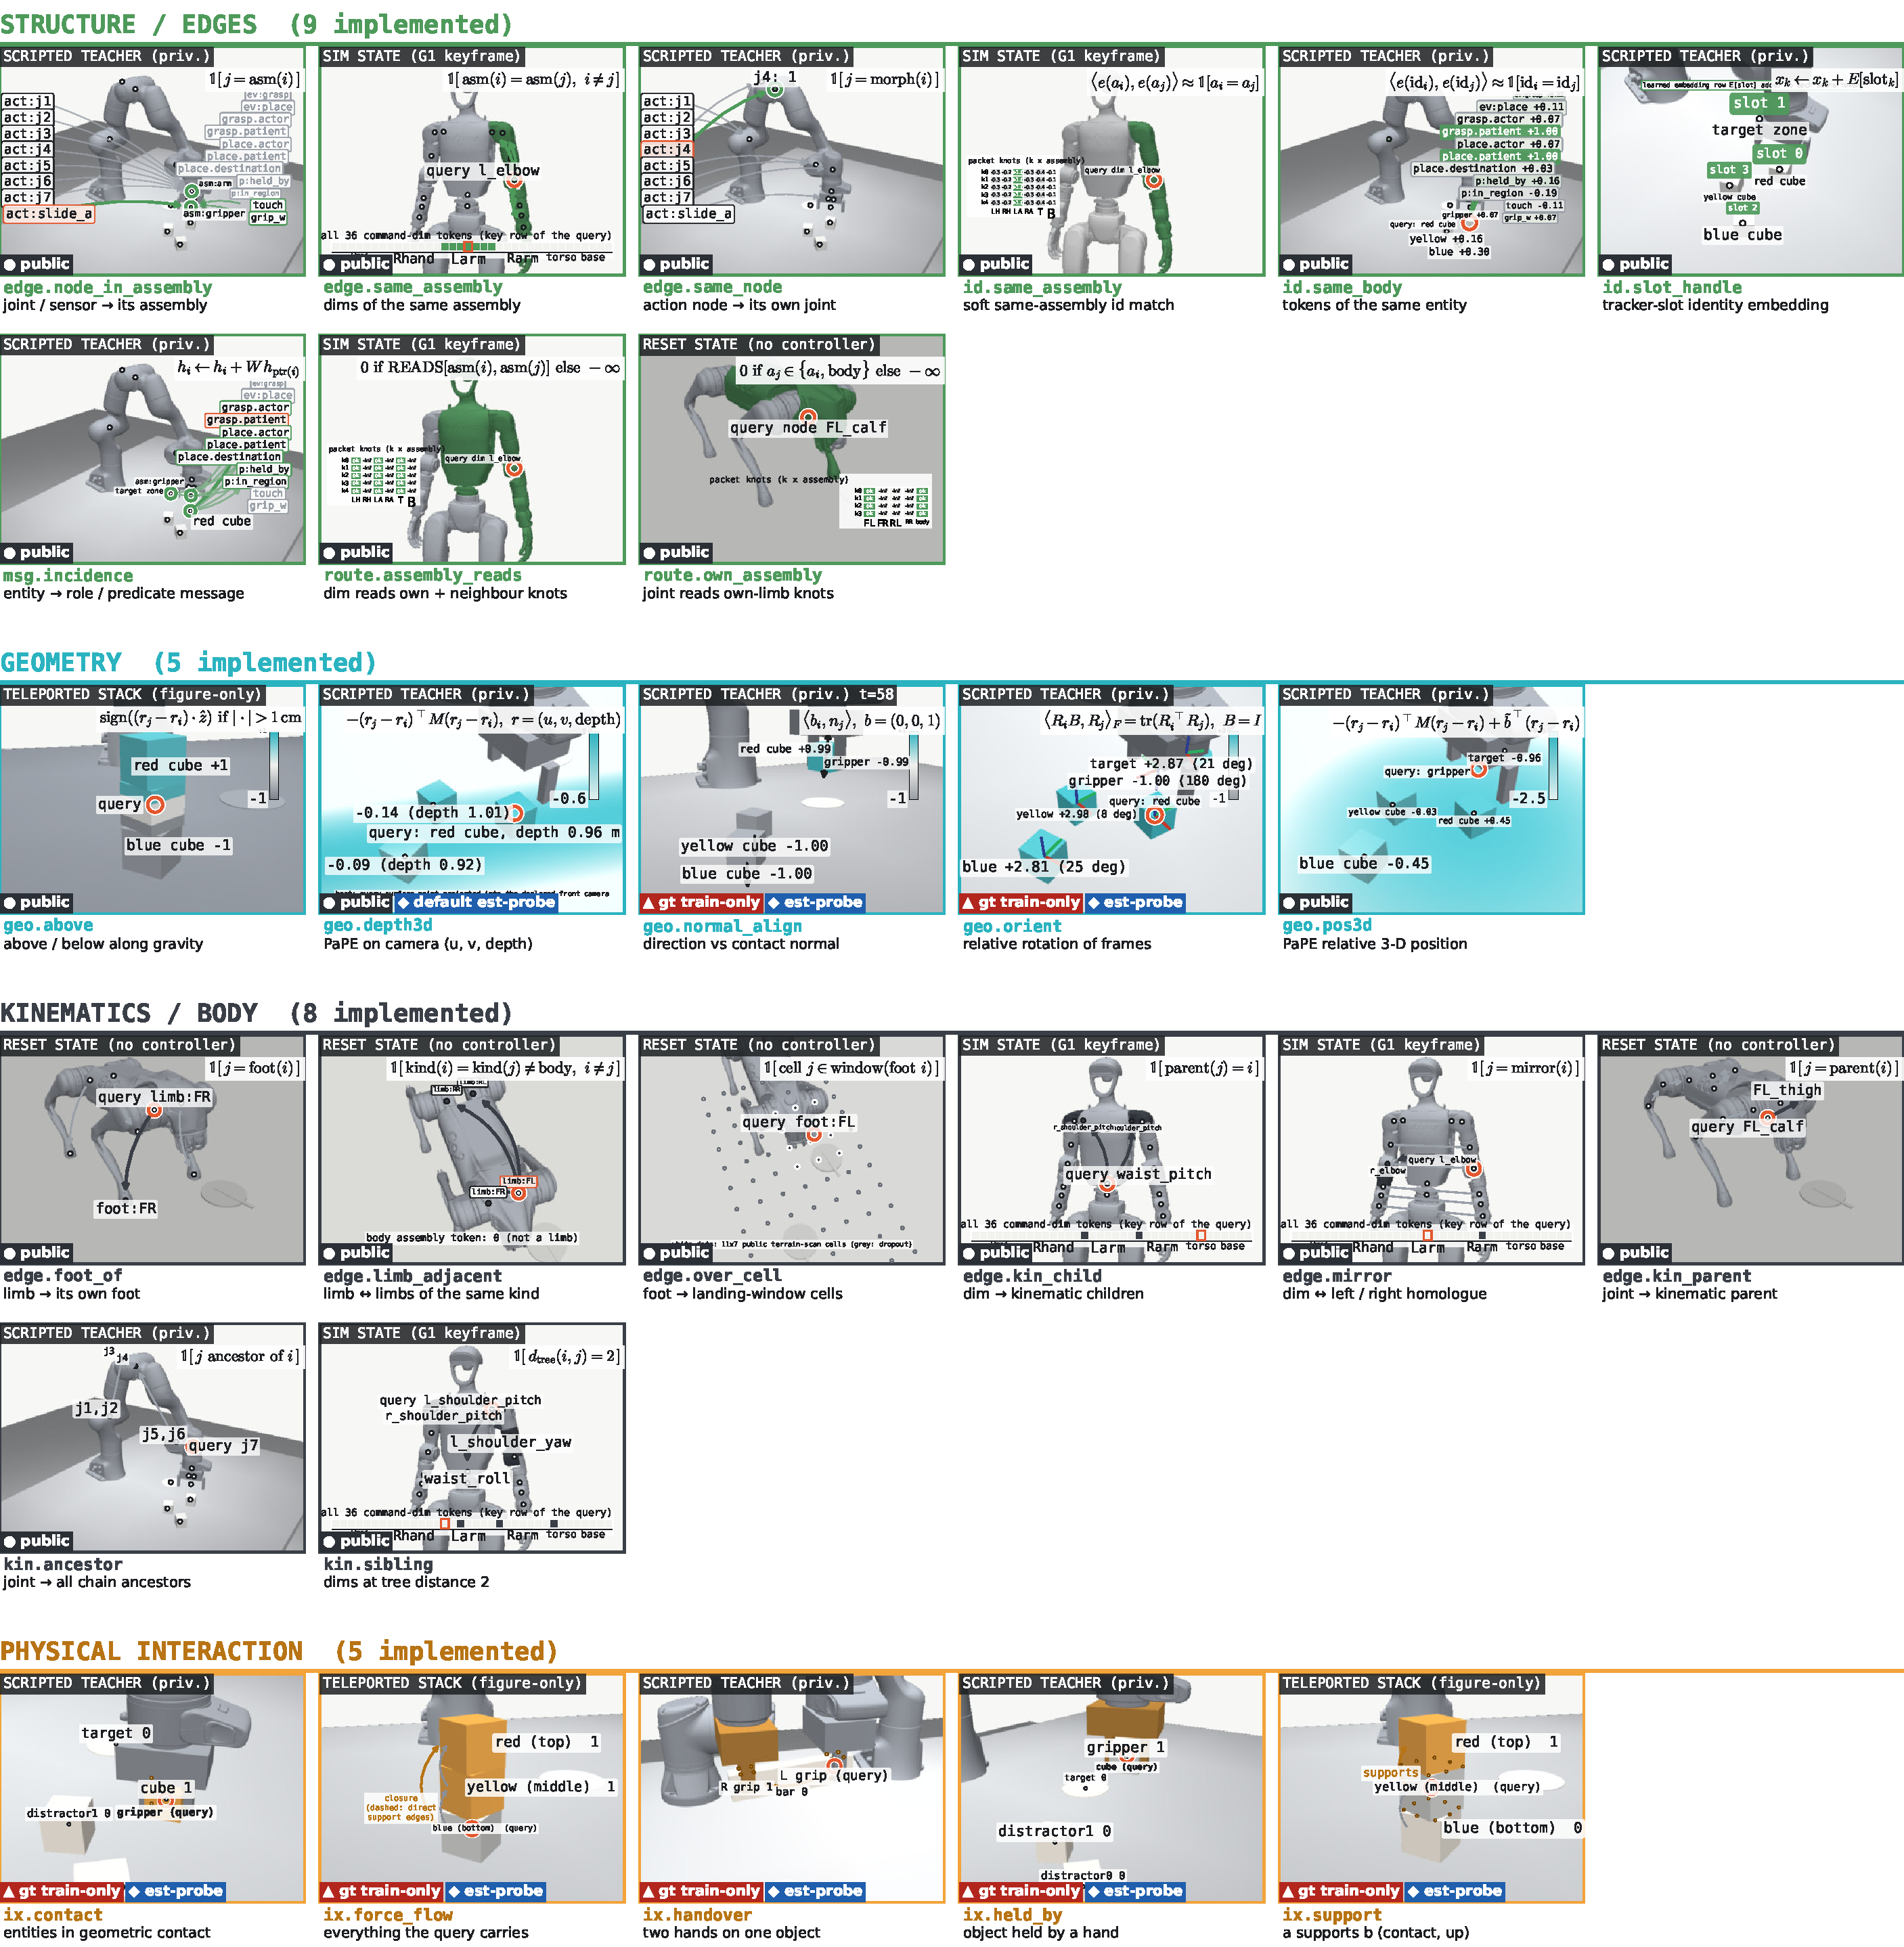
\includegraphics[width=\textwidth]{figures/factor_grid_p1.pdf}
\captionsetup{font=footnotesize}\caption{\textbf{Every implemented relation factor, one tile each} (75 tiles on 5 pages, families in the row order of Table~\ref{tab:relations}). Each tile shows one factor's term for one query token (ring or outlined chip) on a real simulator or environment state, computed by the repository's factor operators or label code; \emph{nothing is trained attention or a trained probe output}. Frame colour = family (Fig.~\ref{fig:fig2}'s four plus structure green); probe readouts are coloured by what they encode (cyan a geometric quantity, amber physical interaction, violet task/procedure state). Top-left chip: scene source (\textsc{scripted teacher} states are privileged). Bottom badge: term source. \emph{public (given)}: computed from public inputs, deployable as shown; \emph{estimated-probe}: the deployed term is the probe's estimate (not shown); \emph{gt \ldots\ training-only}: the colour is the simulator-truth label that trains that probe or readout, never a deployed input. Learned coefficients (edge weights $w$, PaPE $a,b$, rotation/alignment coefficients, same-code gain, task gate) are \emph{set by hand} and stated on the tile. \textsc{illustrative}: \texttt{edge.support\_of} uses a figure-only task-graph variant (no shipped arm/dual graph binds a support role to an entity); \texttt{probe.psi0.grasp\_pt} / \texttt{grasp\_face} show a real replay frame without a label (the replays carry no contact positions). Under each tile: factor, what it encodes, operator and form, source. Generated by \texttt{make\_figures.py tiles}.}\label{fig:tiles}
\end{table*}
\begin{table*}[p]
\captionsetup{type=figure}
\centering
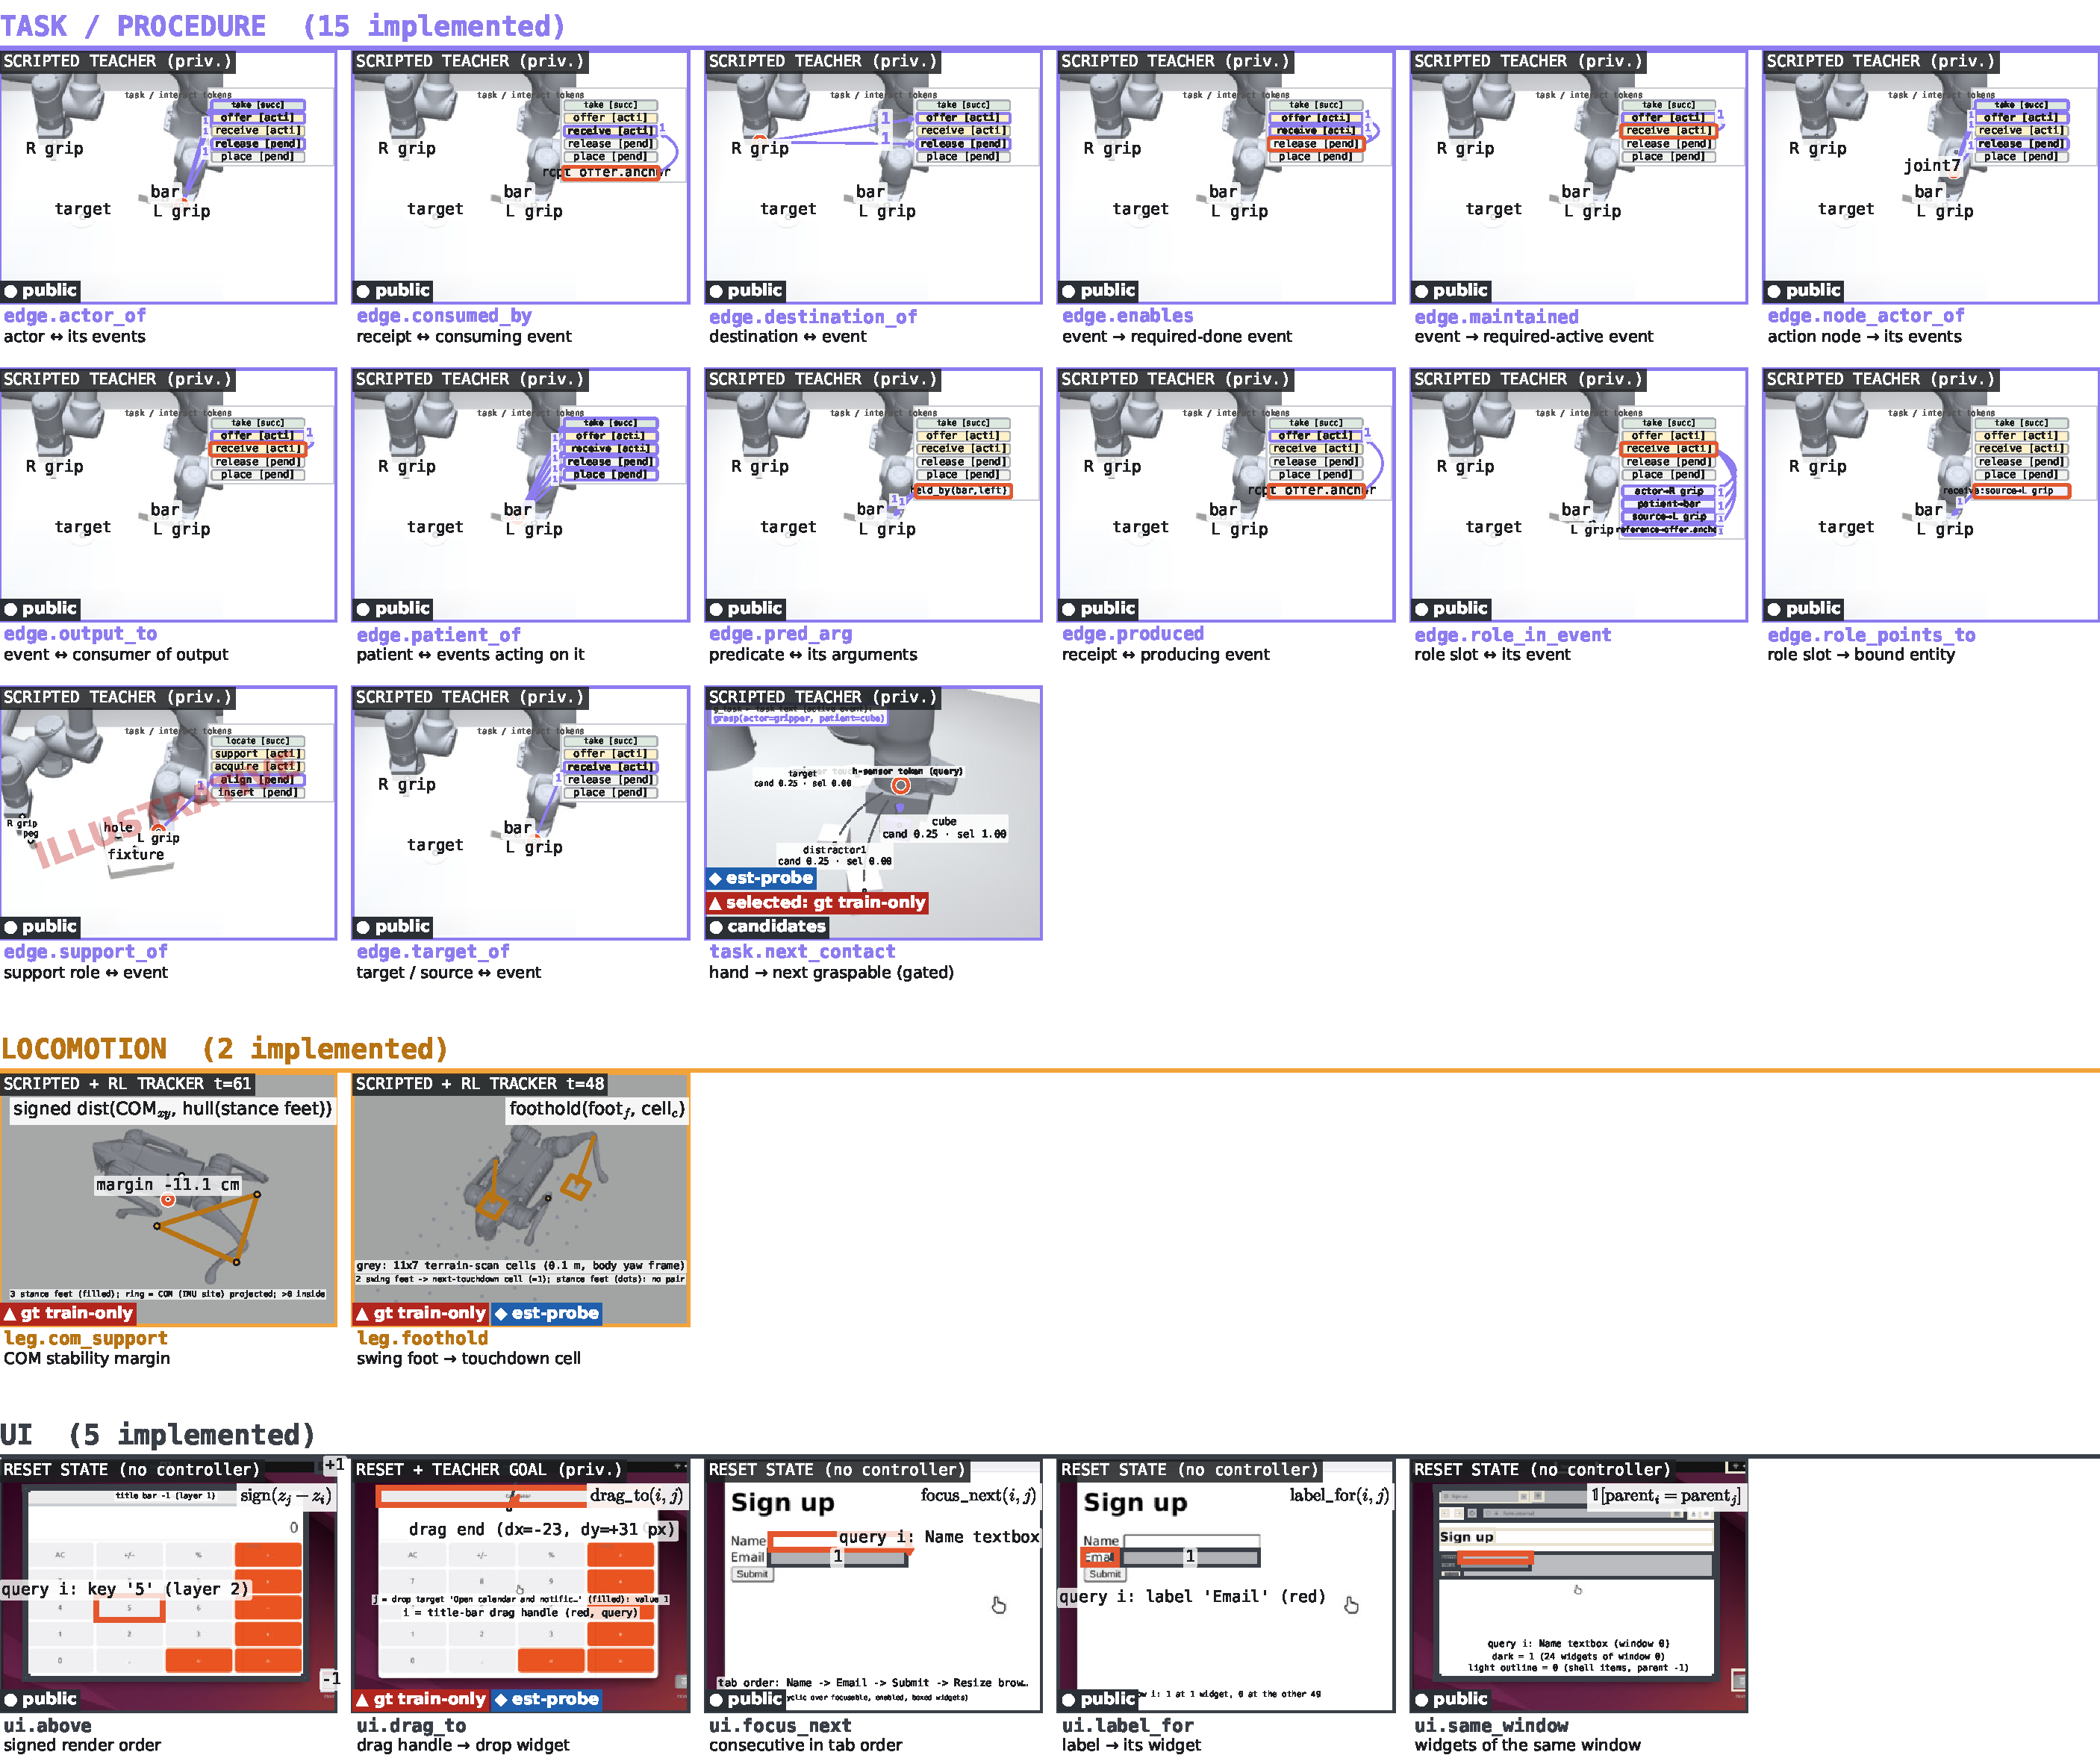
\includegraphics[width=\textwidth]{figures/factor_grid_p2.pdf}
\ContinuedFloat\captionsetup{font=footnotesize}\caption[]{\textbf{Every implemented relation factor} (continued, page 2/5). Badges, colours and marks as on the first page.}
\end{table*}
\begin{table*}[p]
\captionsetup{type=figure}
\centering
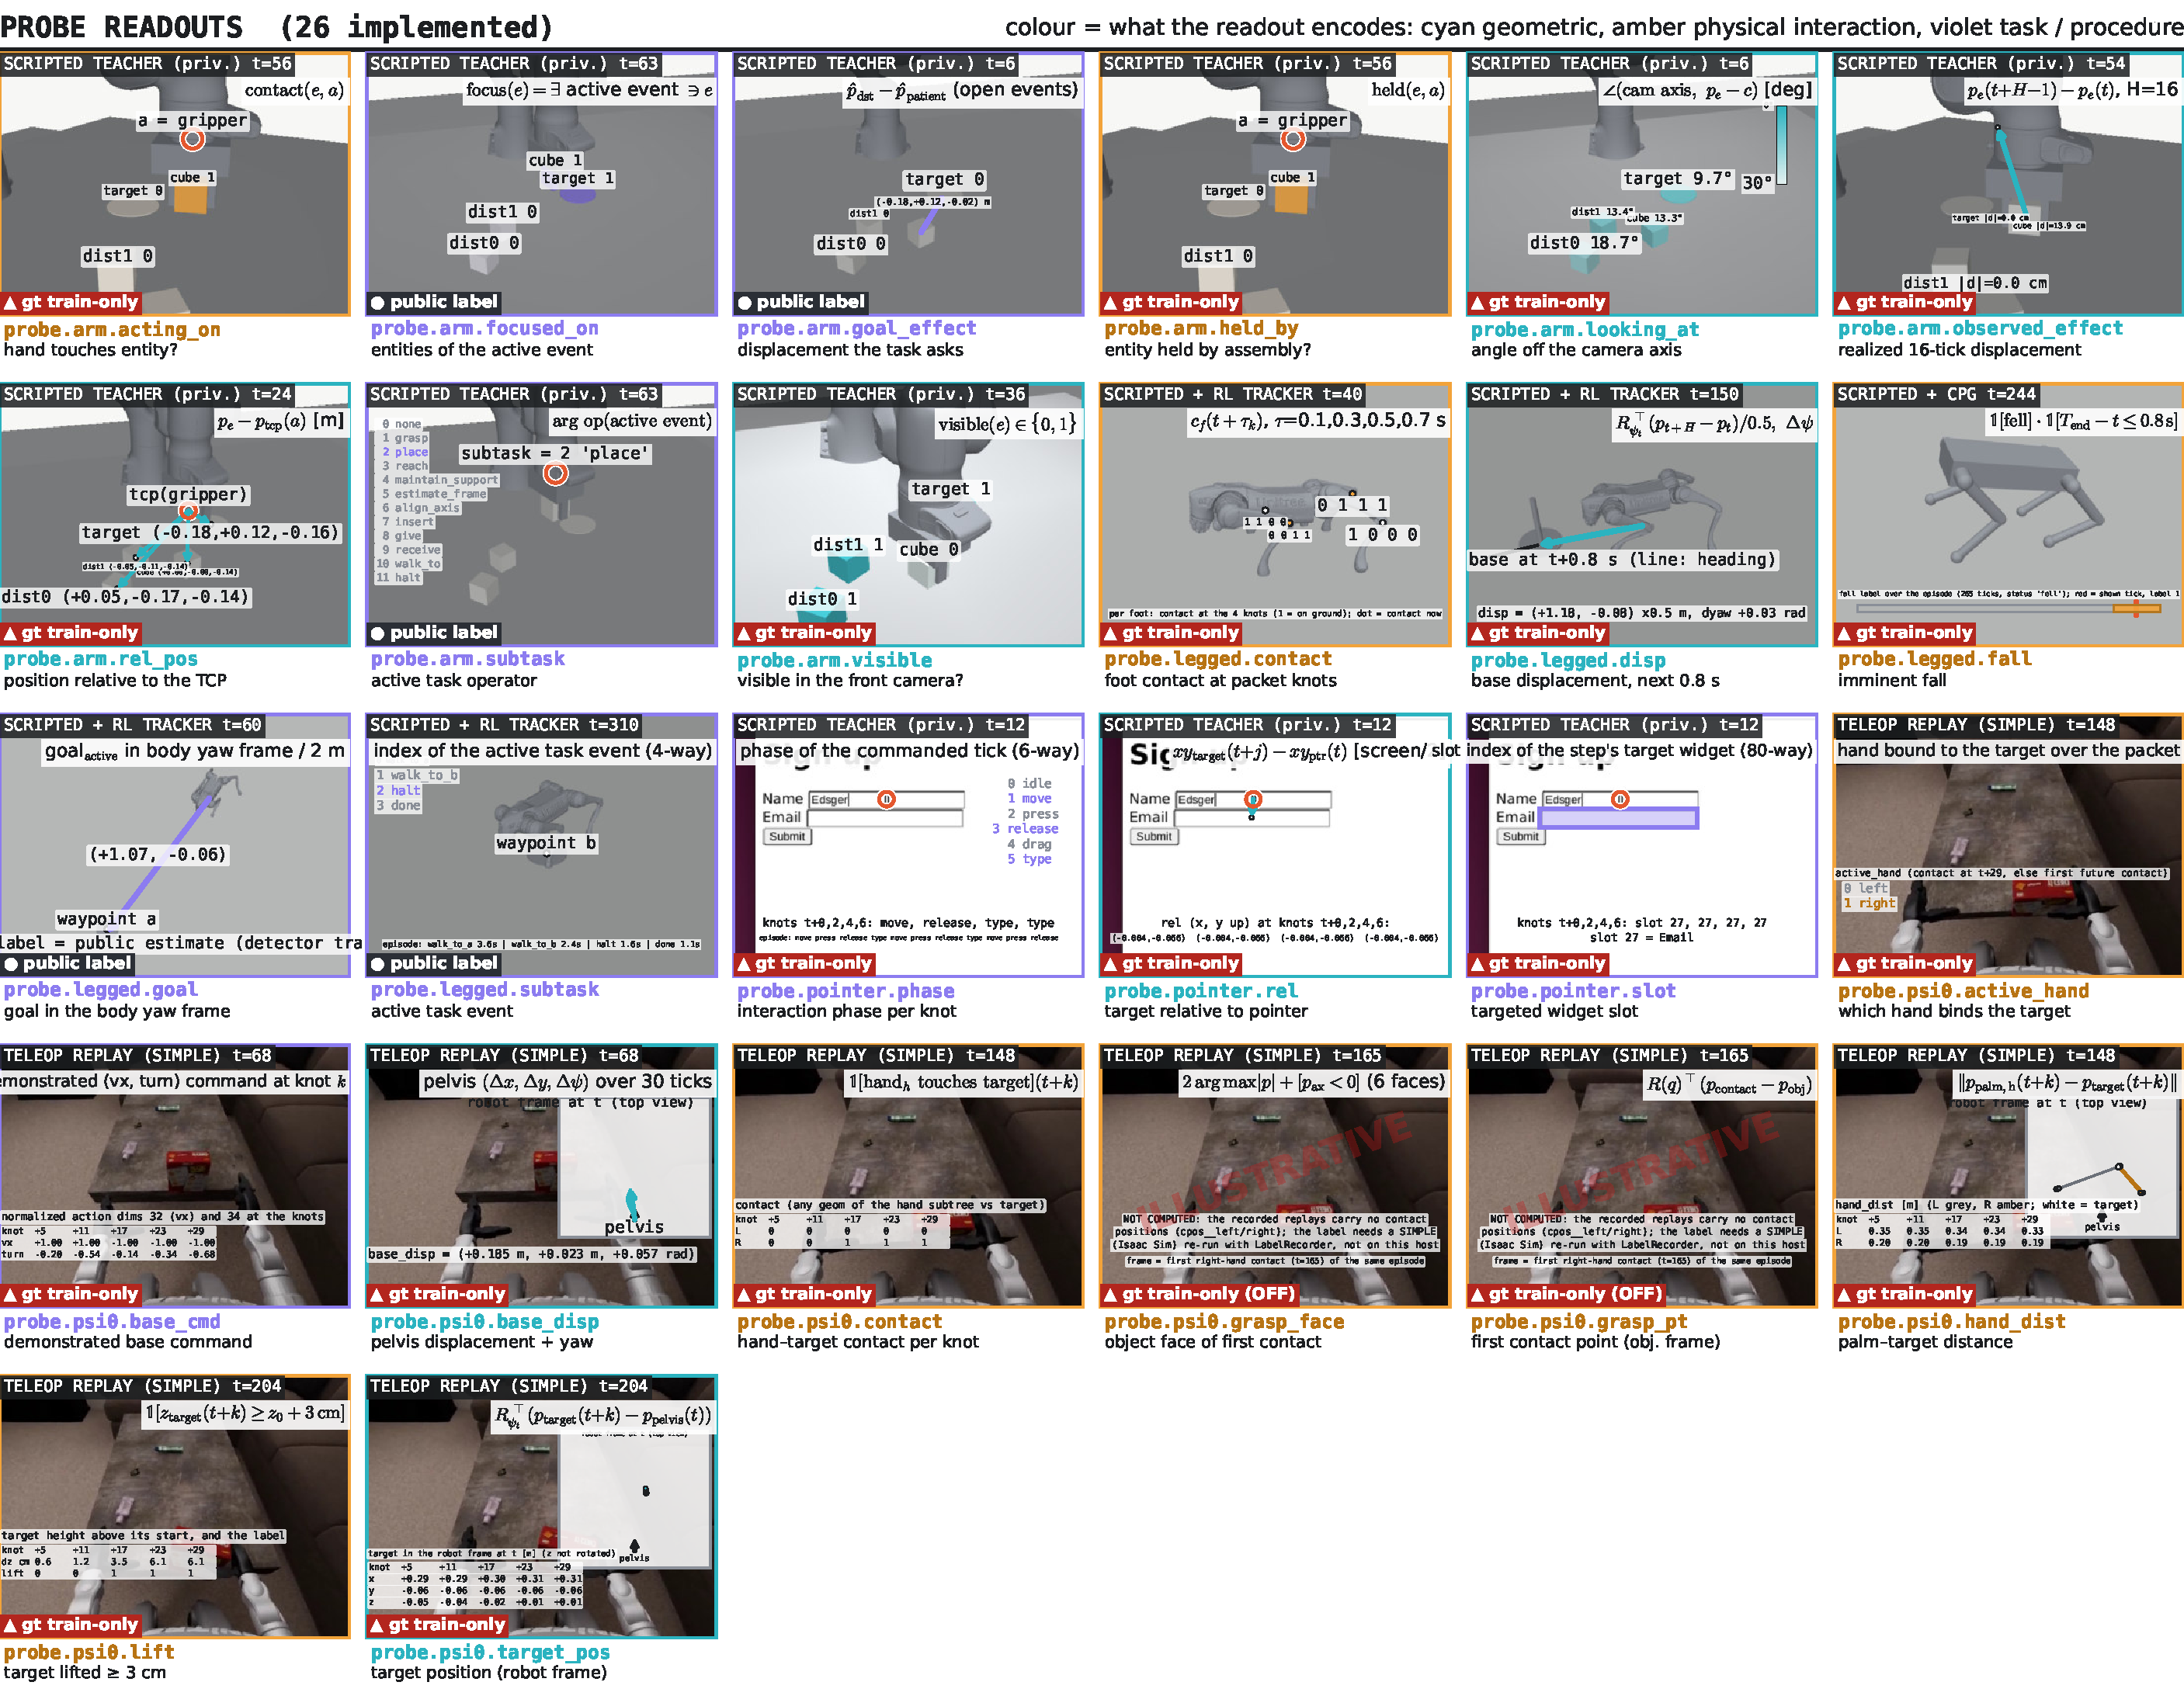
\includegraphics[width=\textwidth]{figures/factor_grid_p3.pdf}
\ContinuedFloat\captionsetup{font=footnotesize}\caption[]{\textbf{Every implemented relation factor} (continued, page 3/5). Badges, colours and marks as on the first page.}
\end{table*}
\begin{table*}[p]
\captionsetup{type=figure}
\centering
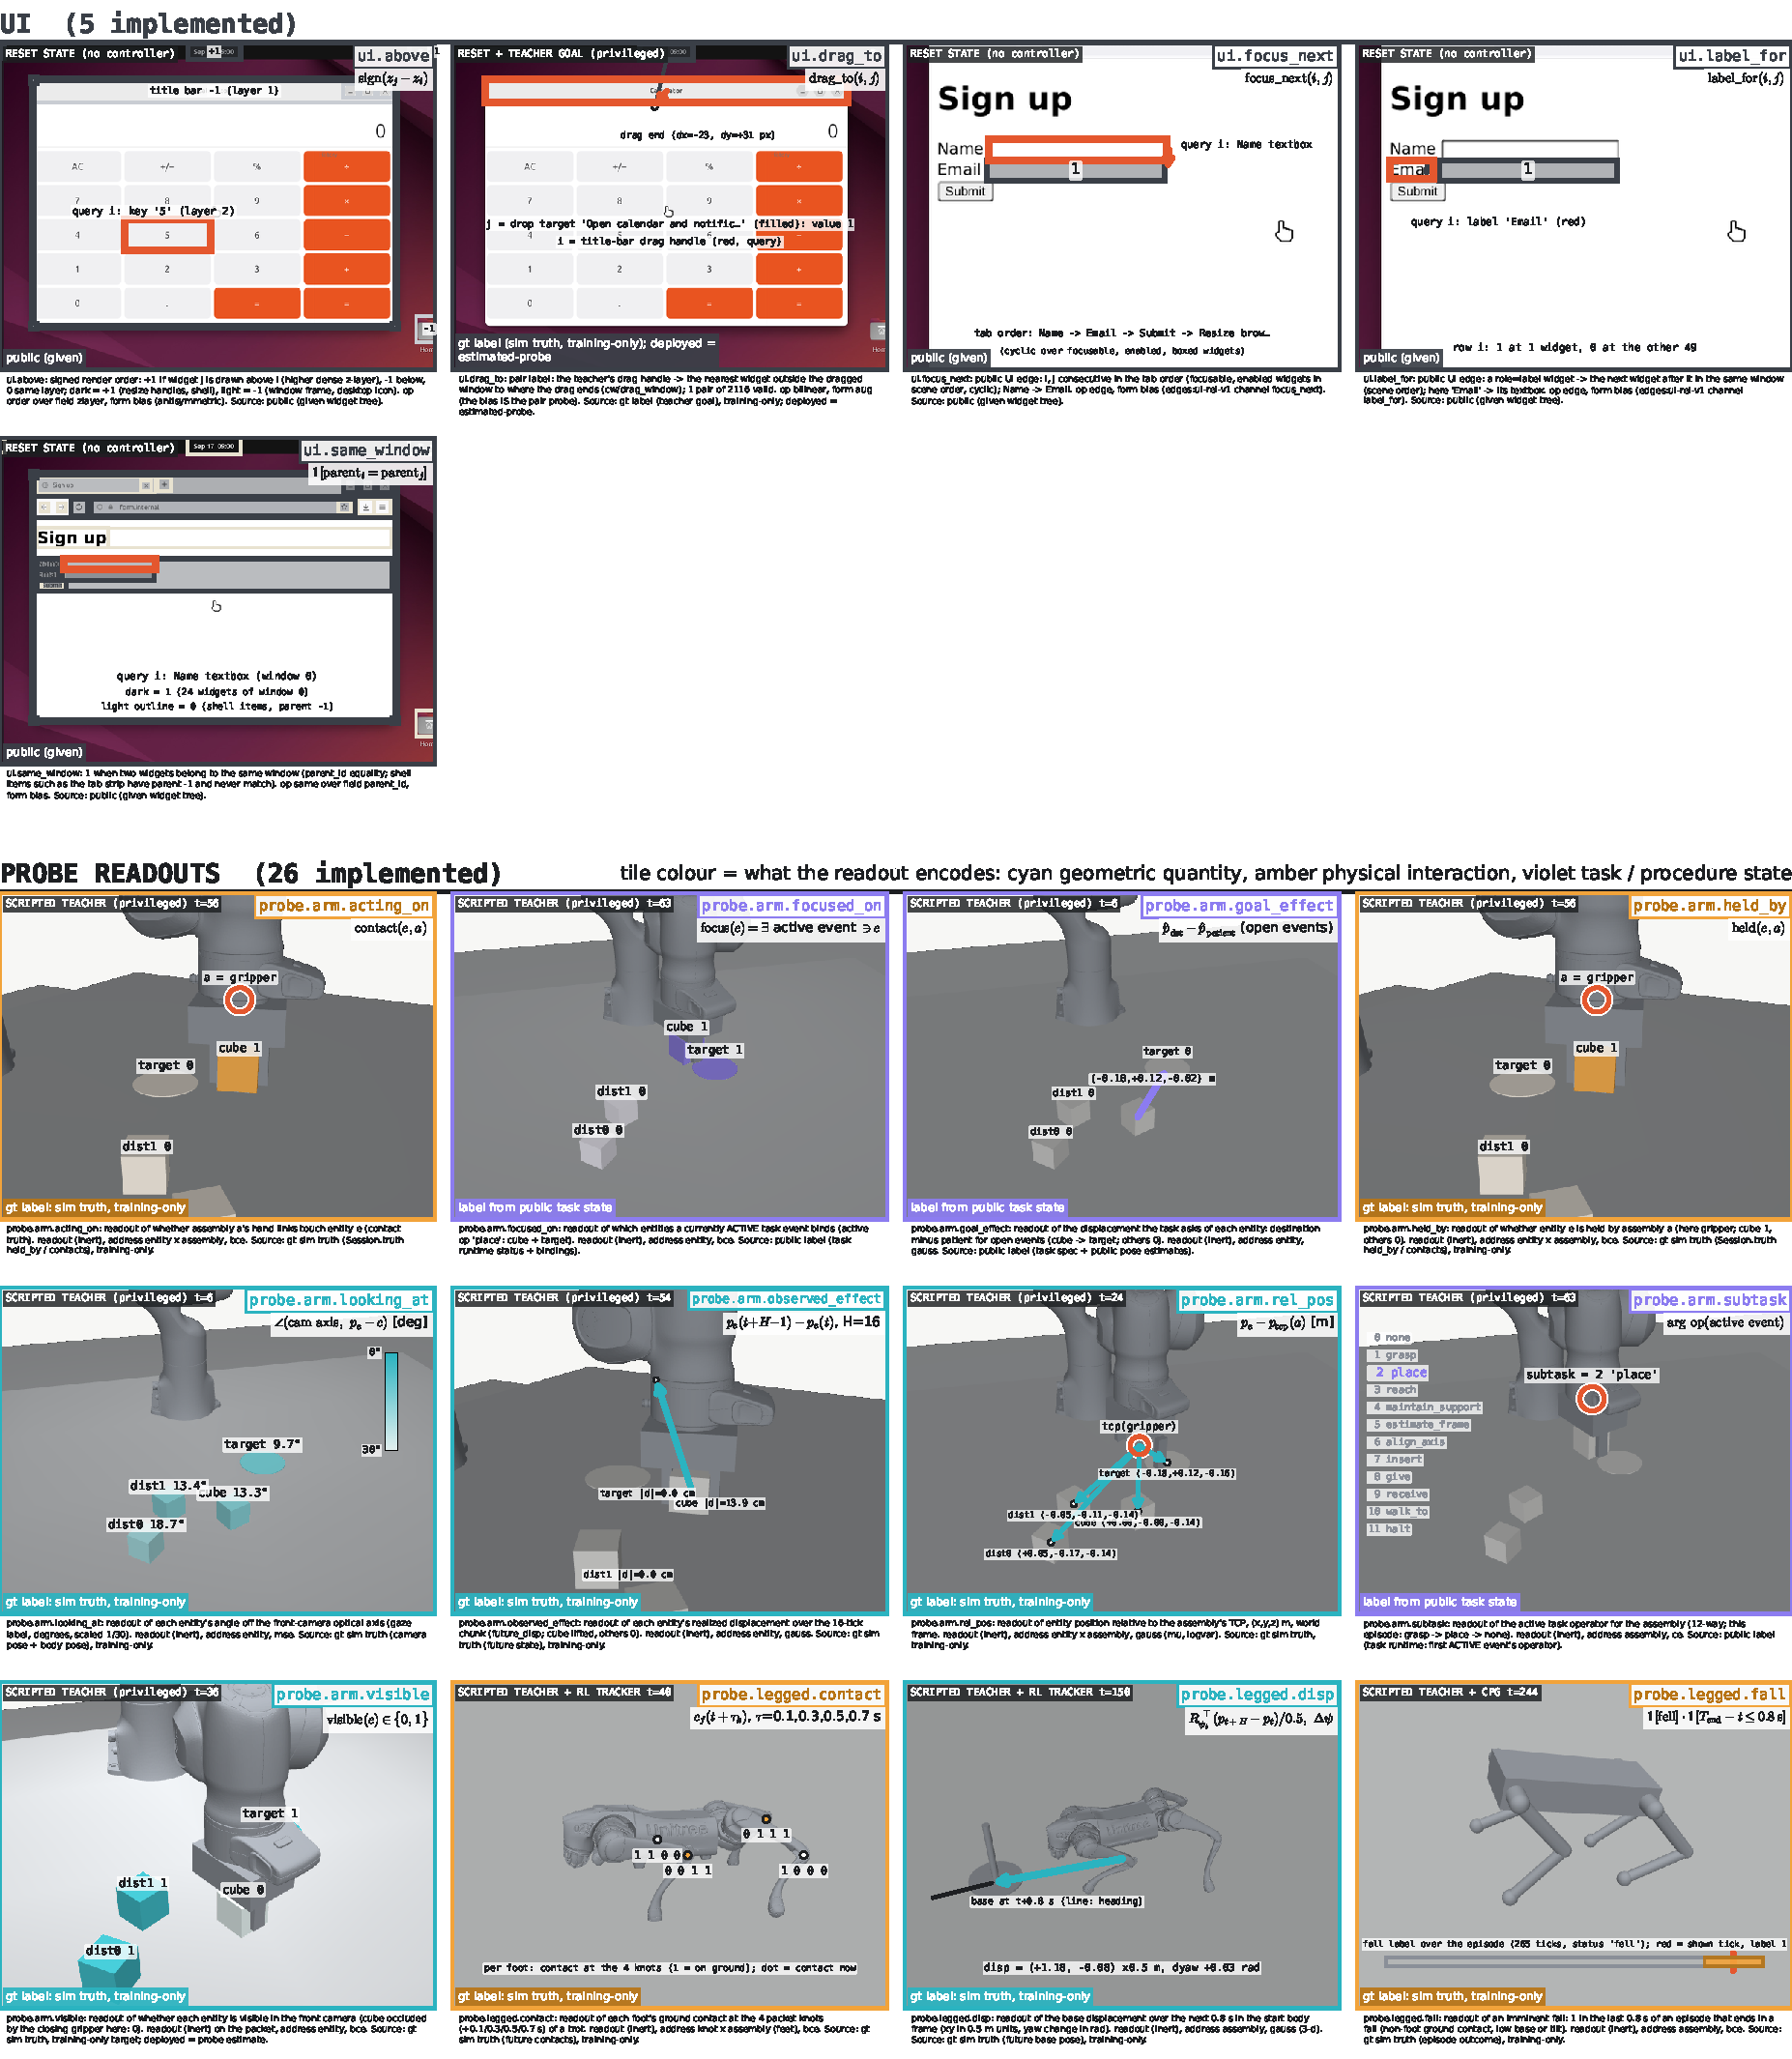
\includegraphics[width=\textwidth]{figures/factor_grid_p4.pdf}
\ContinuedFloat\captionsetup{font=footnotesize}\caption[]{\textbf{Every implemented relation factor} (continued, page 4/5). Badges, colours and marks as on the first page.}
\end{table*}
\begin{table*}[p]
\captionsetup{type=figure}
\centering
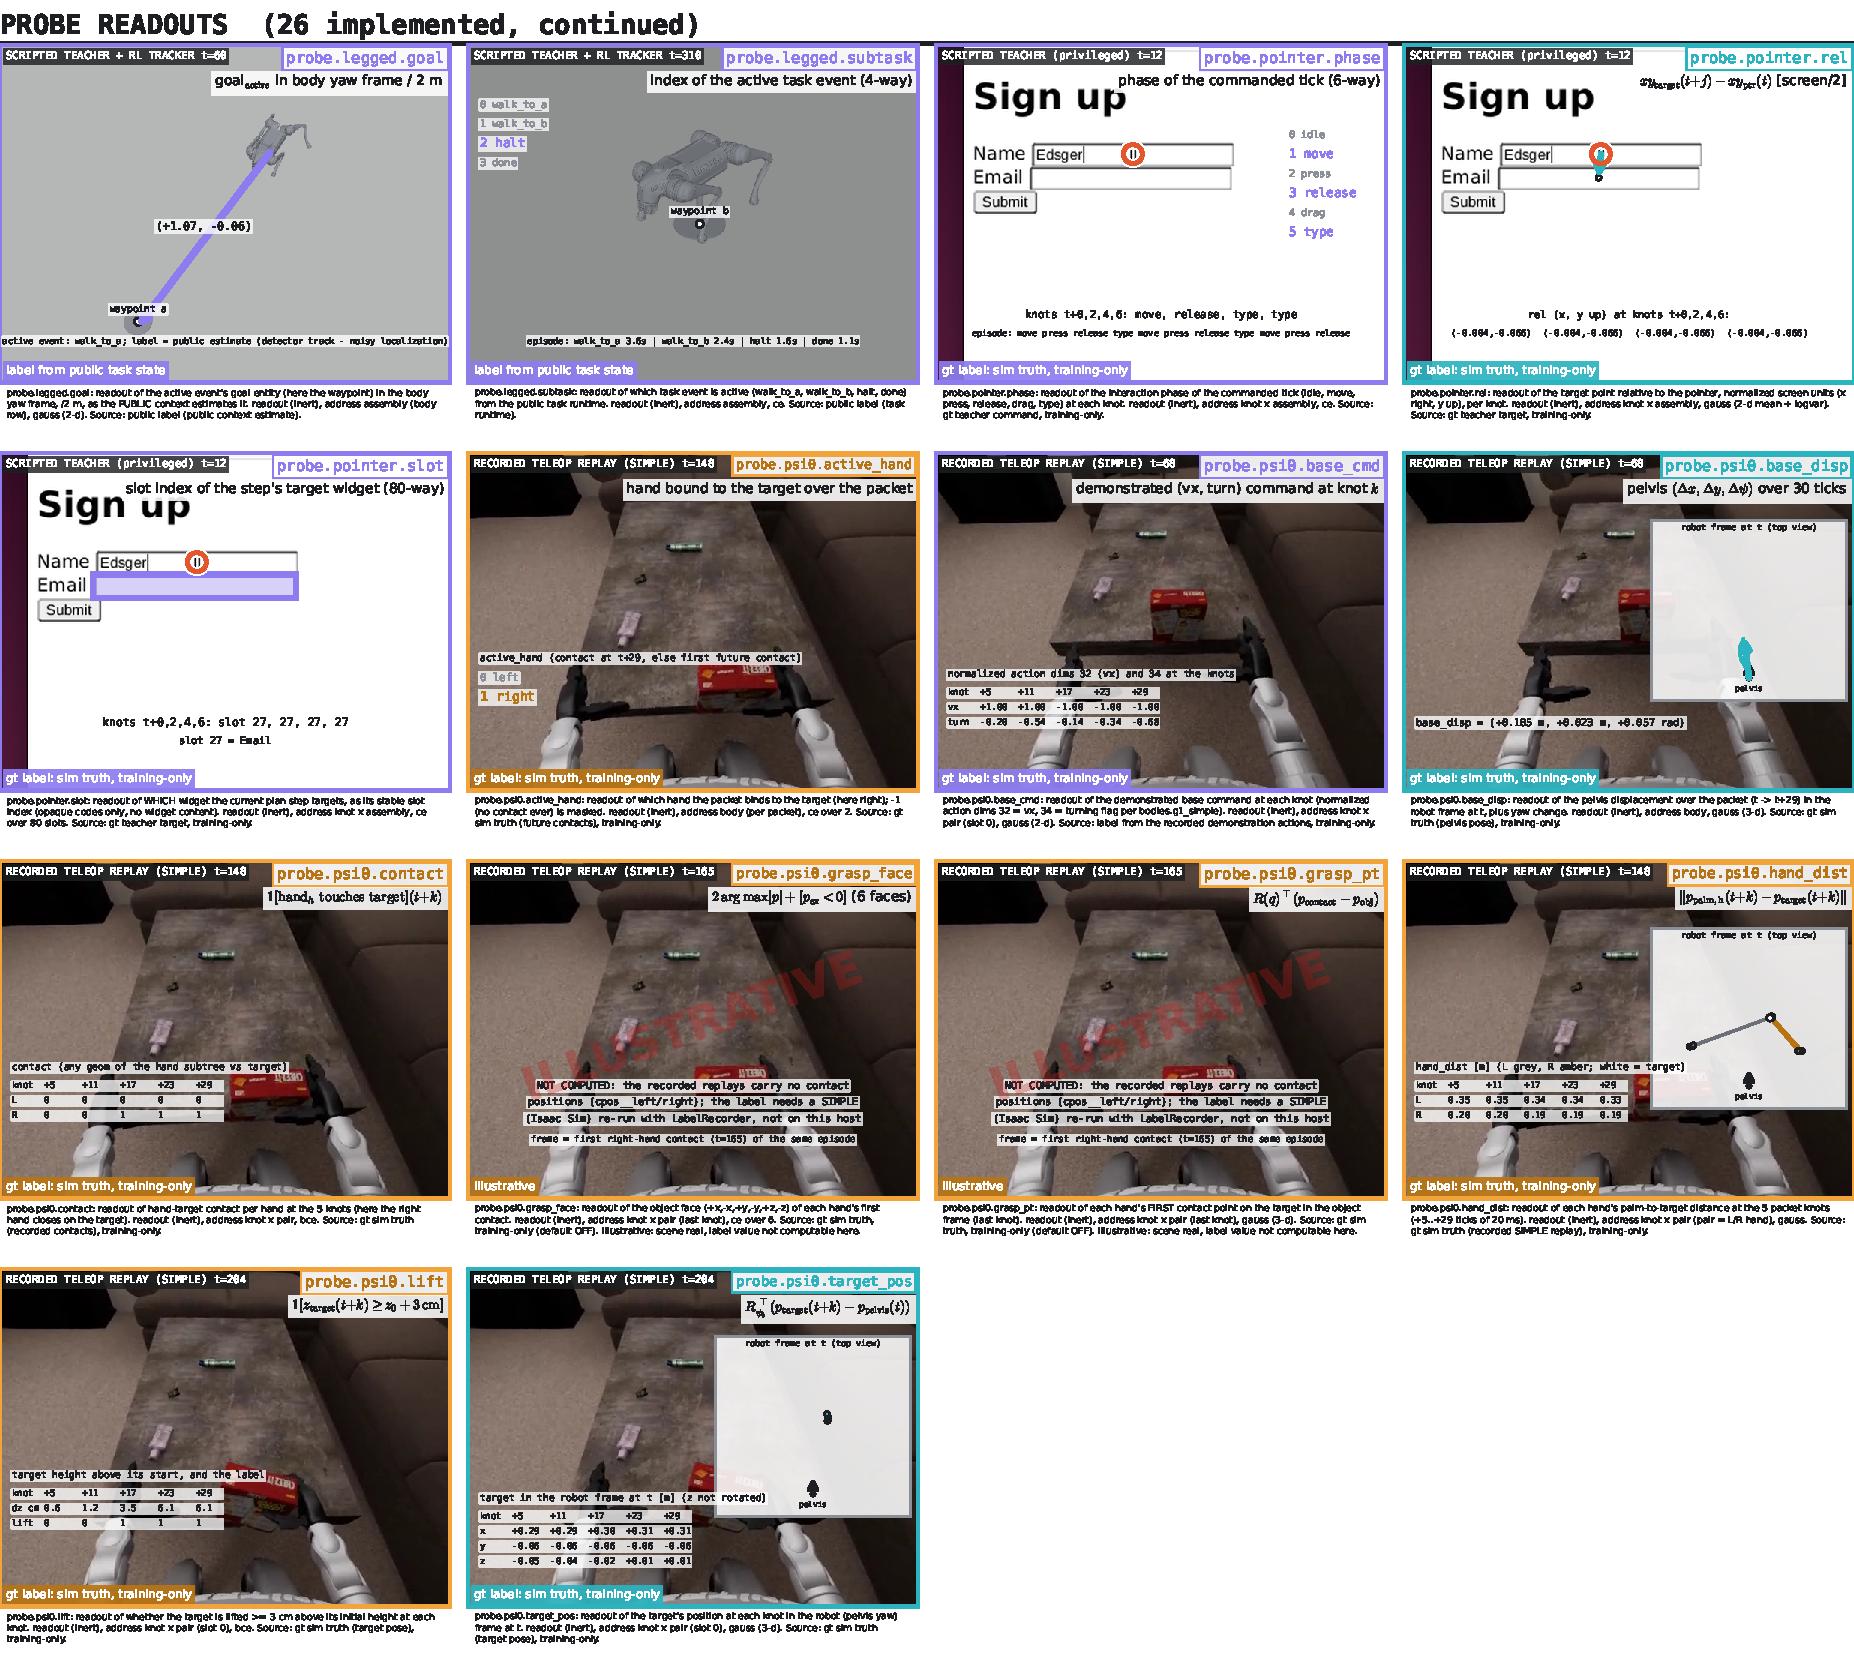
\includegraphics[width=\textwidth]{figures/factor_grid_p5.pdf}
\ContinuedFloat\captionsetup{font=footnotesize}\caption[]{\textbf{Every implemented relation factor} (continued, page 5/5). Badges, colours and marks as on the first page.}
\end{table*}
}

\newcommand{\sysz}{System~0}\newcommand{\sysi}{System~1}\newcommand{\sysii}{System~2}

\title{\vspace{-1.6em}\textbf{Relational attention for a structured semantic latent packet:\\toward morphology-general robot control}}
\author{Jacob Valdez \quad \texttt{\small jacob@commandagi.com}}
\date{\small October 2026}

\begin{document}
\makeatletter
\twocolumn[{\@maketitle\vspace{-1.3em}
\begin{tcolorbox}[colback=rel!9,colframe=rel!60!black,boxrule=0.6pt,arc=2pt,left=6pt,right=6pt,top=3pt,bottom=3pt,halign=center]
{\Large\bfseries\embtotal{} unique simulated embodiments}\\[1pt]
{\scriptsize\color{ink}Counted by \texttt{make\_figures.py embodiments}: distinct body keys built into a simulator model and simulated in at least one recorded run (validation, teacher screen, collection, training or evaluation). \embarms{} single arms (arm $\times$ gripper; \embarmproc{} procedural), \embdual{} dual-arm rigs, \emblegged{} legged and humanoid bodies (\embphum{} procedural humanoids), the $\Psi_0$ G1 and the ComputerWorld pointer (a UI agent, not a robot); \embtrained{} of them are in a training set. All bodies are simulated; none is a physical robot. Breakdown: Table~\ref{tab:embodiments}.}
\end{tcolorbox}\vspace{0.6em}}]
\makeatother

\begin{abstract}\noindent
We study robot control in which a planner (System~1) samples a continuous latent packet $z\in\mathbb{R}^{K\times M\times D}$, one slot per knot time and per body assembly, by rectified-flow matching, and a fast body-side controller (System~0) realizes the same packet as native joint targets from proprioception and touch alone. The packet is supervised to carry task meaning (target, contact, held object, goal) through probes. Every attention layer adds declared relational structure to its logits: the logit is $\langle q_i,k_j\rangle/\sqrt d$ plus a sum of factor terms (PaPE-style relative geometry, kinematic graph, contact, support and force flow, grasp, task-gated next contact, UI structure). The terms come from one declarative registry of 76 factors (75 implemented) that also drives relation-aware data generation and probe readouts, with a deploy guard that keeps simulator truth out of run-time inputs. Across arms, quadrupeds, hexapods, humanoids and a 3D UI world we record that semantic supervision raises arm competence (+0.23 [0.18, 0.28], D-134), carries a task-context halt request into legged behaviour (D-124) and lets packet edits partially steer a pointer (D-142), but that the latent route does not beat behaviour cloning when adapting to a new arm (D-135/D-136). A pre-registered campaign (humanoids, arm diversity, $\Psi_0$, pointer, relation factors) is running. Its recorded outcomes so far are mostly negative or inconclusive: the arm-diversity lineage gate failed; the structured $\Psi_0$ head is below direct fine-tuning on one task (7/20 vs 19/20) and not distinguishable from it on a second (18/20 vs 15/20, $p{=}0.375$); a relation-factor comparison was halted at a floor; and the first humanoid transfer runs are void (two pipeline bugs, now fixed) and are being rebuilt. No humanoid transfer or relation-factor result exists yet; every in-progress node is labelled as such.
\end{abstract}

\begin{tcolorbox}[colback=amber!10,colframe=amber!70!black,boxrule=0.5pt,arc=2pt,left=4pt,right=4pt,top=3pt,bottom=3pt]
\textbf{Status, 5 October 2026.} This is a living report. The training campaign of Sec.~\ref{sec:campaign} is ongoing; results are recorded to the snapshot of 5 Oct 2026 (campaign \texttt{STATUS.md} and decision ledger) and later versions will add to them. Anything marked \emph{in progress} is not a result. Since the 4 Oct version: every humanoid transfer (T5) run made through 4 Oct is \textbf{void} and is being rebuilt (Sec.~\ref{sec:results}); the $\Psi_0$ BendPickMP comparison and the T4 teacher re-gate are recorded.
\end{tcolorbox}

\begin{tcolorbox}[colback=rel!6,colframe=rel!40,boxrule=0.5pt,arc=2pt,left=4pt,right=4pt,top=3pt,bottom=3pt]
\textcolor{rel}{\ding{72}}\;\textbf{Contributions.}\\[1pt]
\pt{1}~\hl{Packet interface.} System~1 $\to z[K{\times}M{\times}D]\to$ System~0, with per-assembly queries computed from public morphology (no per-ID tables); the same tensor is probed, transmitted and consumed.\\
\pt{2}~\hl{Relational attention as a sum of declared terms.} One registry (field $\times$ operator $\times$ form $\times$ source) drives biases, kernel-compatible augmentations, gates and masks, and a deploy guard.\\
\pt{3}~\hl{Relation-aware data.} One privileged state interface, label and scene-part registries, factor-agnostic transforms and a progressive-composition scheduler generate the data each relation needs.\\
\pt{4}~\hl{A ledger.} Recorded results with their intervals, including negative ones, and a pre-registered campaign with its gates.
\end{tcolorbox}

\section{Introduction}
A robot policy that is meant to move between bodies has to say what it intends in a form that survives the change of body. We take the \emph{latent packet} as that form. A planner emits $z$; a body-side controller turns the received $z$ into joint targets using only what the body itself senses. Task meaning therefore has to live on $z$, and we require evidence for that from probes \emph{and} from causal edits of the received packet.

The model is organized by a naming that follows $\Psi_0$~\cite{psi0}: System~2 is an optional frozen vision-language model, System~1 the flow-matching planner, System~0 the packet realizer. Unlike $\Psi_0$'s System~0 (an off-the-shelf RL tracker), ours is a learned realizer; an RL tracker sits underneath it for legged bodies. The second ingredient is a view of attention as a sum of named relational terms. Relative geometry follows the kernel-compatible position terms of PaPE~\cite{pape}; graph, contact and task terms follow the relational-inductive-bias view~\cite{battaglia}. What is new here is bookkeeping: each term is one registry entry that also says which labels train it, which scene parts generate its data and whether it is a bias, an augmentation, a gate, a mask or only a readout.

\paragraph{What this report claims.} (i)~The design, with every factor listed (Table~\ref{tab:relations-summary}, Appendix~A). (ii)~Recorded results from the ledger, each with its decision number and interval (Table~\ref{tab:results}). (iii)~A pre-registered campaign, described as a plan (Table~\ref{tab:campaign}). \emph{Not claimed:} that relation factors help (the experiment that tests this is running), that the latent route transfers across bodies (it did not on a new arm), or any physical-robot result (simulation only).

\begin{figure*}[t]\centering
% Figure 1 (system diagram) for the rrp report. Include with \input{fig1} inside a figure* (full text width) of a 10pt twocolumn article.
% Needs: tikz with arrows.meta, positioning, fit, calc; amsmath. Facts: ~/work/rrp-data/video/intro_v2/model_facts.md, README.md (clocks), code.
\definecolor{s2fill}{HTML}{F3C4CF}\definecolor{s2line}{HTML}{C2577A}
\definecolor{s1efill}{HTML}{F8D9B8}\definecolor{s1eline}{HTML}{D98A3D}
\definecolor{s1dfill}{HTML}{F6C79A}\definecolor{s1dline}{HTML}{C8742A}
\definecolor{s0fill}{HTML}{F6E7A6}\definecolor{s0line}{HTML}{B89A2E}
\definecolor{relcyan}{HTML}{2BB3C0}\definecolor{depgreen}{HTML}{5CC98A}
\definecolor{ink}{HTML}{3A3F47}
\resizebox{\textwidth}{!}{%
\begin{tikzpicture}[font=\scriptsize,>={Stealth[length=3.2pt]},
  blk/.style={draw=#1,line width=1.1pt,rounded corners=3pt,align=center,inner sep=3pt},
  s2/.style={blk=s2line,fill=s2fill,dashed},
  s1e/.style={blk=s1eline,fill=s1efill},
  s1d/.style={blk=s1dline,fill=s1dfill},
  s0/.style={blk=s0line,fill=s0fill},
  trn/.style={draw=ink!60,fill=ink!6,dashed,line width=0.8pt,rounded corners=3pt,align=center,inner sep=3pt},
  note/.style={font=\tiny,align=center,text=ink},
  clk/.style={font=\tiny\itshape,text=ink!85},
  flow/.style={->,thick,ink},
  rel/.style={->,thick,relcyan}]
% ---- inputs
\node[note,anchor=east] (imgin) at (0.2,3.0) {camera image\\+ instruction};
\node[s2,text width=33mm] (s2) at (3.0,3.0) {\textbf{System 2} \emph{(optional)}\\frozen VLM + resampler\\$\to$ 16 image tokens};
\draw[flow,dashed,s2line] (imgin) -- (s2);
\node[note,anchor=south] at (1.3,1.05) {public / estimated tokens};
\foreach \i/\n in {0/morph,1/scene,2/task,3/interact}{
  \node[s1e,minimum width=19mm,minimum height=4.6mm,inner sep=1pt,line width=0.8pt] (bank\i) at (1.3,0.55-\i*0.55) {\n};}
\node[note,anchor=north,text width=30mm] at (1.3,-1.45) {arm: objects, task graph\\legged: joints, terrain cells\\pointer: widgets, instruction};
% ---- System 1
\node[s1e,text width=28mm,minimum height=22mm] (enc) at (4.9,0) {\textbf{encoder}\\[1pt]typed banks, self-attn with\\\textcolor{relcyan}{\textbf{relation bias}}\\[1pt]\tiny run once per observation};
\node[s1d,text width=50mm,minimum height=22mm] (dec) at (10.0,0)
  {\textbf{decoder} over packet slots $(k,m)$\\[1pt]
   $x_{k,m}\!=\!z_{\mathrm{in}}\!+\!\mathrm{node}(\mathrm{asm}_m)\!+\!\mathrm{node\_from\_ctx}(\mathrm{morph}_m)\!+\!h_k$\\[1pt]
   cross-attn to cached context, $\tau$-conditioned};
\draw[s1dline,line width=0.6pt,rounded corners=4pt] ([shift={(-2mm,-2.6mm)}]enc.south west) rectangle ([shift={(2mm,2.4mm)}]dec.north east);
\node[font=\scriptsize\bfseries,text=s1dline,anchor=north east] at ([shift={(1.5mm,-2.8mm)}]dec.south east) {System 1 (flow matching)};
\node[note] (eps) at (10.0,3.0) {noise $\varepsilon$};
\draw[flow] (eps) -- (dec.north |- 0,1.5);
\node[note,anchor=west,text width=50mm,align=left] at (10.15,2.25) {rectified flow, Euler $n_{\mathrm{fe}}{=}8$;\\all $K{\times}M$ tokens denoised in parallel};
\draw[flow] (bank0.east) -- ++(0.35,0) |- ([yshift=3mm]enc.west);
\draw[flow] (bank3.east) -- ++(0.35,0) |- ([yshift=-3mm]enc.west);
\draw[flow,s2line,dashed] (s2.east) -| node[right,pos=0.8,note,text=s2line,align=left]{image tokens\\(scene bank)} (enc.north);
\draw[flow] (enc) -- node[above,note,pos=0.5]{K,V} (dec);
% ---- packet
\begin{scope}[shift={(14.2,0)}]
  \foreach \k in {0,1,2,3}{\foreach \m in {0,1,2}{
    \pgfmathsetmacro{\sh}{20+18*mod(\k*2+\m*3,5)}
    \fill[relcyan!\sh!white,draw=relcyan!80!black,line width=0.4pt] (\k*0.42-0.84,0.42-\m*0.42-0.19) rectangle ++(0.38,0.38);}}
  \node[font=\tiny,text=ink,anchor=south] at (0,0.78) {knots $k$};
  \node[anchor=north,align=center,text=relcyan!55!black,inner sep=1pt] (zlab) at (0,-0.95) {\textbf{packet} $z\!\in\!\mathbb{R}^{K\times M\times D}$\\[-1pt]\tiny arm: $K{=}4$, $D{=}64$};
\end{scope}
\draw[relcyan,line width=1pt,rounded corners=3pt] (13.0,-0.85) rectangle (15.4,1.1);
\draw[flow] (dec.east) -- (13.0,0);
% ---- System 0
\node[s0,text width=34mm,minimum height=22mm] (s0) at (18.1,0)
  {\textbf{System 0} (realizer)\\[1pt]node queries from $q,\dot q$, touch,\\IMU (own senses); cross-attend\\packet knots, mask \texttt{route.own\_assembly}\\[1pt]\tiny no task, scene or image input};
\draw[flow] (15.4,0) -- node[above,note,yshift=1pt]{$z$} (s0.west);
\node[s0,fill=s0fill!40,line width=0.8pt,text width=30mm] (pd) at (18.1,-3.4) {PD / joint tracker $\to$ MuJoCo body};
\draw[flow] (s0.south) -- node[right,note,xshift=1pt]{joint targets} (pd.north);
\draw[flow] (pd.east) -- ++(0.9,0) |- node[near end,above,note]{} ([yshift=3mm]s0.east);
\node[note,anchor=west,align=left] at (21.0,-1.6) {$q,\dot q$,\\touch,\\IMU};
% ---- deploy boundary and training-only band
\draw[depgreen,line width=1.4pt,dash pattern=on 5pt off 3pt] (-0.4,-2.75) -- (15.7,-2.75);
\node[font=\tiny\bfseries,text=depgreen!55!black,anchor=south west] at (-0.4,-2.73) {deploy boundary: above, public and estimated inputs only};
\node[trn,text width=40mm] (tenc) at (7.3,-3.95) {\textbf{target encoder $E$} (training only)\\demonstrated future actions\\$\to$ target packet $z^{\star}$};
\draw[->,thick,ink!60,dashed] (tenc.north) -- (tenc.north |- 0,-1.95) -- (8.2,-1.95) -- (8.2,-1.12);
\node[trn,text width=22mm] (lab) at (11.0,-3.95) {\textbf{labels} (sim truth)};
\node[trn,text width=30mm] (probe) at (14.2,-3.95) {\textbf{probes} read $z$\\[-1pt]\tiny contact, goal, held object, \dots};
\draw[rel,dashed] (zlab.south |- 0,-1.62) -- node[right,note]{} (probe.north);
\node[note,anchor=east] at (7.15,-2.25) {flow target $z^{\star}$};
\draw[->,thick,ink!60,dashed] (lab) -- (probe);
\node[note,font=\tiny\bfseries,text=depgreen!45!black,anchor=north east] at (13.9,-2.8) {labels (sim truth) $\to$ probes, training only};
% ---- clocks
\node[clk,font=\scriptsize\itshape,anchor=north west,text width=215mm,align=left] at (-0.4,-5.3)
  {clocks. arm: System 1 replans every 0.4\,s (4 knots), System 0 at 20\,Hz, physics 500\,Hz. legged / humanoid: replan every 20 ticks (0.4\,s), System 0 at 50\,Hz.};
\end{tikzpicture}}
\caption{\textbf{System overview.} System~1 encodes typed context tokens (public or estimated fields only) once per observation and denoises the packet $z$ in parallel; System~0 realizes the same $z$ from the body's own senses with no task, scene or image input. Dashed boxes are optional (System~2) or training-only (target encoder, labels, probes: simulator truth, never a deployed input).}
\label{fig:iface}
\end{figure*}


\section{Architecture}
\paragraph{System~1.} An encoder--decoder transformer trained by rectified flow~\cite{rectflow,fm}. The encoder reads clean context tokens once per observation. Tokens come in typed banks: \emph{morph} (one per action node, passive joint and assembly), \emph{scene} (tracked objects with uncertainty and an explicit null token), \emph{task} (events, role bindings, predicates, status) and \emph{interact} (touch and receipts). Legged and humanoid bodies use one global token plus per-joint, per-limb, per-foot and terrain-cell tokens; the pointer world uses UI-widget and instruction-character tokens. Only the $\Psi_0$ family and an optional arm variant read an image, through System~2 (a frozen VLM and a small resampler giving 16 image tokens).

The decoder's queries are the packet slots $(k,m)$ for knot $k$ and assembly $m$,
\begin{equation}
\begin{aligned}x_{k,m}={}&z_{\tau}[k,m]\,\text{in-proj}\\&+\mathrm{node}(a_m)+\mathrm{node\_from\_ctx}(c_m)+h_k,\end{aligned}
\label{eq:query}
\end{equation}
where $a_m$ are the assembly's public morphology features, $c_m$ its encoded morph token and $h_k$ a knot embedding. The identity of a query is thus computed from public morphology, not looked up in a per-ID table, which is what lets a new body produce new queries. Each block applies self-attention over time and across assemblies, cross-attention to the cached context and an MLP, conditioned on flow time $\tau$. Sampling integrates $\tau:0\to1$ by $8$ Euler steps over \emph{all} $K\times M$ tokens in parallel; the loss is $\lVert v-(z-\epsilon)\rVert^2$ with $z_\tau=(1-\tau)\epsilon+\tau z$. A training-only target encoder $E$ turns demonstrated future actions into the target packet; probes read meaning out of $z$ and supervise it.

\begin{table}[t]\centering\small
\caption{\textbf{Packet shape per family} ($z[K{\times}M{\times}D]$), from the code. Pointer $D{=}26$ with the v2 key code (T8).}\label{tab:packet}
\setlength{\tabcolsep}{3.5pt}
\begin{tabular}{@{}lcccl@{}}\toprule
family & $K$ & knot times / horizon & $M$ & $D$\\\midrule
arm / dual & 4 & 0.1--0.7\,s & 1 / 2 & 64\\
legged / humanoid & 4 & 0.1--0.7\,s (0.8\,s) & $\le$11 & 32\\
$\Psi_0$ (G1) & 5 & chunk steps 5--29 (0.6\,s) & 6 & 64\\
pointer & 4 & -- & 1 & 16 (26)\\\bottomrule
\end{tabular}
\end{table}

\paragraph{System~0.} Each control tick, one query per actuated node is built from public morphology and the \emph{current} measured state ($q,\dot q$; legs add IMU, own-foot touch and an oscillator). The node queries cross-attend to the packet's knot tokens, whose times are shifted by the elapsed phase, through the routing mask \code{route.own\_assembly} (a node reads only its own assembly's knots; legged bodies add the body assembly's); then self-attention among nodes and an MLP give one normalized joint target per node. System~0 receives \emph{no} task, instruction, scene, image or System~1 state: task meaning arrives only through $z$, sensor feedback every tick. Clocks: the arm replans every 0.4\,s and runs System~0 at 20\,Hz over 500\,Hz physics; legged and humanoid bodies replan every 0.4\,s with a 0.8\,s packet at 50\,Hz.

\paragraph{Deploy boundary.} Every token set separates \code{fields} (public or estimated) from \code{labels} (simulator truth). Each field and factor carries a provenance, \emph{public}, \emph{estimated} (a public estimator or the factor's own probe) or \emph{privileged}, and a deployable policy refuses privileged sources (\code{assert\_deployable}). Ground truth trains the probes; at run time only public and estimated values steer attention.

\section{Relational attention bias}
Every attention call in the model uses one shared multi-head attention whose logit is
\begin{equation}
\begin{aligned}A_{ij}={}&\frac{q_i^{\top}k_j}{\sqrt d}+\sum_{f\in\mathcal{B}}w_{f,h}\,\gamma_f\,v_f(i,j)\\&+\big\langle\phi_q(i),\phi_k(j)\big\rangle\;\big(-\infty\text{ if masked}\big),\end{aligned}
\label{eq:logit}
\end{equation}
where each registered factor $f$ contributes one term $v_f(i,j)$ in one \emph{form}: an additive \emph{bias} ($f\in\mathcal B$), a kernel-compatible \emph{augmentation} appended to $q,k$ (the $\langle\phi_q,\phi_k\rangle$ term, so fused attention kernels still apply), a \emph{gate} $\gamma_f=2\sigma(u\cdot c+b)$ that scales another term by a task, goal or embodiment summary $c$, or a hard \emph{mask}. Three non-attention forms (message, embed, readout) reuse the same entries. Every learned coefficient is zero-initialized, so switching a factor on in a trained model is a no-op at step~0.

\paragraph{Operators.} A factor is an entry over about a dozen operators, which are the only code per relation \emph{kind}: \code{diff}, \code{sqdiff+diff} (PaPE), \code{rel\_rot}, \code{align}, \code{order}, \code{same}, \code{sim}, \code{edge}, \code{hop}, \code{ancestor} (closure), \code{flow}, \code{bilinear} and \code{unary}. The PaPE term in its compact kernel-compatible form is
\begin{equation}
v_{\mathrm{PaPE}}(i,j)=-(r_j-r_i)^{\top}M_i(r_j-r_i)+\tilde b_i^{\top}(r_j-r_i),
\label{eq:pape}
\end{equation}
with $M_i\succeq0$ diagonal in a learned frame and $\tilde b_i$ a learned direction; it splits into a \emph{distance} part and a \emph{direction} part (the first two panels of Fig.~\ref{fig:fig2}). Graph terms come from declared morphology (\code{kin.ancestor}, siblings, same assembly) and from the supplied task graph (actor, patient, destination edges). Pair terms that cannot be read from public inputs (contact, support, held-by, handover, next contact) are \code{bilinear}: $\langle U x_i,Vx_j\rangle$ is at once the attention term and the pair probe, so the bias \emph{is} a supervised attention subspace, and its estimate can feed a graph factor (\code{ix.support}$\to$\code{ix.force\_flow}) with source \emph{probe}, deployable. \code{task.next\_contact} is gated by the task so that the same scene shows several candidate edges and the bias narrows to the one the task needs.

\paragraph{Sites and controls.} Factors attach at the encoder (\code{ctx>ctx}), decoder cross- and self-attention (\code{act>ctx}, \code{act>act}) and System~0 routing (\code{node>knot}). Uniform controls apply to any factor: \code{off}, \code{zero}, \code{rewired} (keys permuted, degree preserving), \code{shuffled}, \code{reversed}, and for message factors \code{serialized}, the same facts as hashed text (the equal-information baseline).

\paragraph{Probes and diagnostics.} Probes are readouts in the same registry. Attention maps and probe accuracy are diagnostics: causal use is shown by editing the packet or the context and rolling out (Section~\ref{sec:results}, D-142, D-124). Fig.~\ref{fig:fig2} shows factor \emph{values} computed from real simulator states, not learned attention; Fig.~\ref{fig:tiles} covers every factor.

\begin{figure*}[t]
\centering
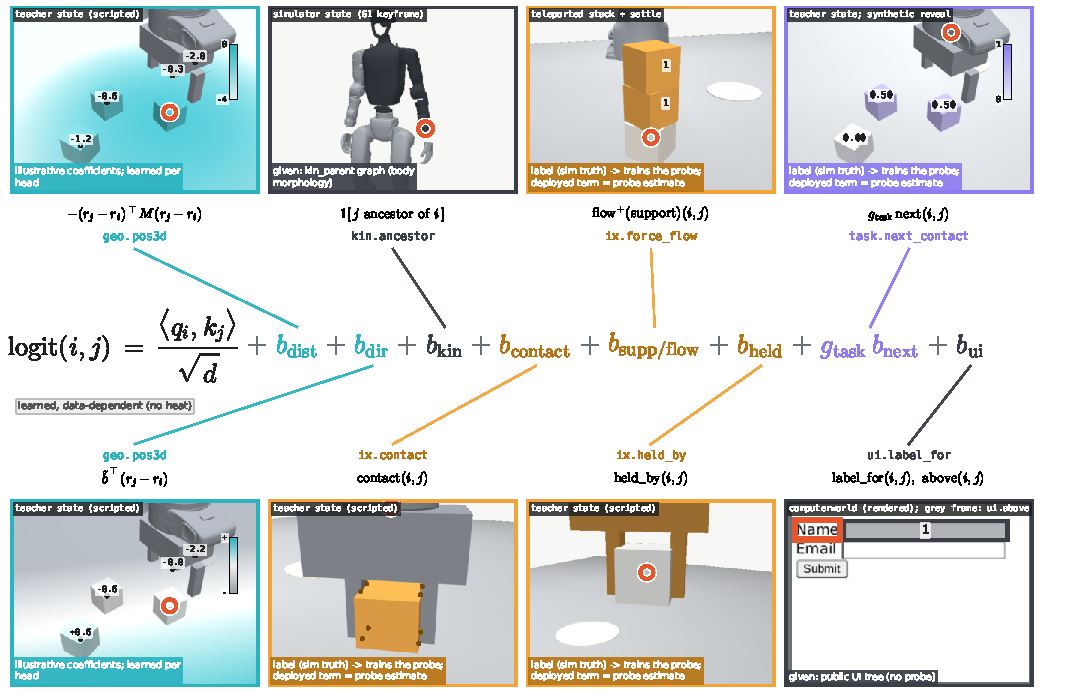
\includegraphics[width=\textwidth]{figures/fig2.pdf}
\caption{\textbf{The attention logit, one term at a time.}
Each panel stretches one term of $\mathrm{logit}(i,j)$ for a single query token (ring) over a real simulator state; frame colour is the relation family
(geometry, kinematics/UI, contact/support/grasp, procedure). The content term $\langle q_i,k_j\rangle/\sqrt{d}$ is learned and data-dependent, so it has no panel.
\emph{The values shown are computed by the factor operators of \texttt{rrp.policies.relations} on real simulator states; they are not trained attention.}
Panels 1--2 run the PaPE kernel with hand-set, illustrative coefficients (the model learns them per head); panels 3 and 8 are public, given structure (G1 kinematic tree; computerworld widget tree).
For probe-sourced pair terms (panels 4--7) the colour shows the simulator-truth label that trains the probe; the deployed term is the probe's estimate, which is not shown.
Scenes: scripted-teacher Panda pick-and-place states (1, 2, 4, 6, 7), a teleported three-cube stack (5), a G1 keyframe (3), a rendered desktop UI (8).
Terms whose form is \emph{aug} (\texttt{geo.pos3d}, \texttt{ix.contact}, \texttt{ix.held\_by}, \texttt{task.next\_contact}) enter the logit as $\langle\phi_q(i),\phi_k(j)\rangle$ in Eq.~(\ref{eq:logit}); the panel shows that value. Planned relation factors (e.g.\ \texttt{time.same\_track}) are omitted.}
\label{fig:fig2}
\end{figure*}

\relsummary

\section{Relation-aware data and curriculum}
Each relation may need data that decouples one invariance, so data generation is as declarative as the factors. A single privileged \code{StateView} (capability \code{privileged\_truth}, implemented per backend) exposes poses, contacts, joints, cameras and UI trees for \emph{supervision only}. Four registries sit on it: \code{LABELS} (18 label functions, each with a provenance \code{gt}, \code{task} or \code{estimator}), \code{PARTS} (7 composable scene components: \code{table\_objects}, \code{camera\_depth}, \code{grasp\_target}, \code{stack}, \code{terrain\_steps}, \code{cw\_viewport}, \code{cw\_depth}, each declaring the dynamics it activates, requires and conflicts with), \code{TRANSFORMS} (6 factor-agnostic sample transforms: \code{reveal}, \code{surprise}, \code{cf\_swap}, \code{noise}, \code{occlude}, \code{subsample}) and one composition operator that returns a scene covering a requested set of active dynamics. A factor entry names its \code{label} and its \code{gen} parts or transforms; decoupling pairs are copies of a scene that differ only in one factor's value.

\paragraph{Progressive composition.} One scheduler samples the generated rows. Every factor starts at composition depth $k{=}1$ (isolated parts); it is promoted to $k{+}1$ when its competence $c_f\ge\theta_f$ for two consecutive intervals; per-factor shares are $\propto s_{\min}+s_f$, clipped to $[2\%,35\%]$, with struggle $s_f=(1-c_f)+0.5\,p_f+i_f+e_f$ (plateau, interference and attributed failures); the full-task share follows a rising floor. Steering is a small grammar (boost, pin, freeze, drop, revert) logged for exact replay. \emph{State:} implemented and plumbing-smoked; the campaign run that measures competence by depth and interference (T9) is in progress, so there is no curriculum result in this report. The \code{cf\_swap}, \code{reveal} and \code{surprise} transforms produce the decoupling and progressive-information variants of the contact and next-contact labels.

\section{Environments, bodies and tasks}
All simulation is native MuJoCo~\cite{mujoco} with robot models largely from MuJoCo Menagerie~\cite{menagerie} (plus a batched Warp legged env and the $\Psi_0$ SIMPLE benchmark on Isaac Sim) behind one environment, one policy and one task interface; one harness runs any accepted policy $\times$ environment $\times$ task triple and records declined pairs with reasons. Table~\ref{tab:envs} lists the bodies and tasks and Fig.~\ref{fig:envs} shows one frame of each environment. Evaluation routes use matched seeds: R0 scripted teacher (privileged), R1 oracle packet $E(\text{expert chunk})$ (diagnostic, not deployable), R2 generated packet (deployable), plus a behaviour-cloning (BC) positive control and task-context edit suites. Splits are sealed before results.

% generated by make_figures.py table_envs from rrp code and frozen splits; do not edit
\begin{table*}[t]\footnotesize\setlength{\tabcolsep}{2.5pt}\renewcommand{\arraystretch}{1.1}
\caption{Environments, bodies, tasks, the relation families whose factors resolve in each env's net family (implemented factors: total, net-side + probe), and the status of each track.}
\label{tab:envs}
\begin{tabular}{@{}>{\raggedright\arraybackslash}p{0.12\textwidth}>{\raggedright\arraybackslash}p{0.30\textwidth}>{\raggedright\arraybackslash}p{0.22\textwidth}>{\raggedright\arraybackslash}p{0.10\textwidth}>{\raggedright\arraybackslash}p{0.18\textwidth}@{}}
\toprule
env & bodies & tasks & relation family & status \\ \midrule
arm \newline\scriptsize\ttfamily mujoco/\allowbreak{}arm & panda, sawyer, ur10e, ur5e, vx300s, parm5/6/7 variants (5), 24 procedural pa2s* (pg2 / tf3 grippers); sealed targets panda\_\allowbreak{}tf3, xarm7 & pick\_\allowbreak{}place, reach\_\allowbreak{}pose & arm\newline 42 (33+9) & teacher + learned; transfer split primary\_\allowbreak{}v1 / armdiv \\
dual \newline\scriptsize\ttfamily mujoco/\allowbreak{}dual & two mounted arms (pairs of the arm pool) or one dual body & support\_\allowbreak{}insert, handover, assign\_\allowbreak{}left, assign\_\allowbreak{}right, pivot\_\allowbreak{}against\_\allowbreak{}surface & dual\newline 43 (34+9) & parked, D-146: eval of external checkpoints; scripted teachers only \\
quad \newline\scriptsize\ttfamily mujoco/\allowbreak{}legged & go2, anymal\_\allowbreak{}c, a1, hexapod6, pquad4, sprawl4, sprawl8, hexapod6\_\allowbreak{}long & waypoint\_\allowbreak{}contact, foothold\_\allowbreak{}steps & legged\newline 21 (16+5) & teacher + frozen tracker \\
humanoid \newline\scriptsize\ttfamily mujoco/\allowbreak{}legged & t1, g1, h1, op3, apollo, adam\_\allowbreak{}lite, talos + phum procedural & 9 h\_\allowbreak{}* tasks (h\_\allowbreak{}steps, h\_\allowbreak{}gap, h\_\allowbreak{}walk, \ldots{}); held out: h\_\allowbreak{}steps\_\allowbreak{}carry, h\_\allowbreak{}gap\_\allowbreak{}cart & humanoid\newline 21 (16+5) & teacher + frozen tracker; campaign in progress \\
tracker \newline\scriptsize\ttfamily warp/\allowbreak{}legged & same legged and humanoid bodies, GPU-batched & locomotion, h\_\allowbreak{}steps, h\_\allowbreak{}gap & legged / humanoid\newline (as above) & tracker training only \\
SIMPLE \newline\scriptsize\ttfamily simple & g1\_\allowbreak{}simple (G1, 36-d command) & 6 G1Wholebody* tasks & psi0\newline 19 (10+9) & $\Psi_0$ SIMPLE on Isaac Sim; path-traced renderer caveat; step-1 reproduced on 3 of 6 tasks \\
CWorld \newline\scriptsize\ttfamily computer\allowbreak{}world & cw\_\allowbreak{}pointer (cursor, keys) & calc\_\allowbreak{}sum, open\_\allowbreak{}type, drag\_\allowbreak{}window, fill\_\allowbreak{}form & pointer\newline 10 (7+3) & scripted teacher; procedural strings v3 \\
\bottomrule
\end{tabular}
\end{table*}


\begin{figure*}[t]
\centering
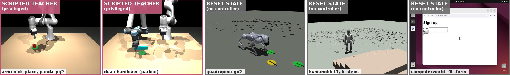
\includegraphics[width=\textwidth]{figures/fig3_envs.pdf}
\caption{\textbf{The five environments.} One rendered frame each. The arm and dual-arm frames are mid-episode states of the scripted teacher (privileged source); the quadruped, humanoid and computerworld frames are reset states with no controller running, so they show the scene, not a rollout.}
\label{fig:envs}
\end{figure*}

% Section 6. Fragment. Needs table_results.tex input in the main file (placed here for float order).
\section{Results so far}\label{sec:results}
Table~\ref{tab:results} lists every result recorded to the snapshot of 5 Oct 2026, with the setting, the comparison and the interval recorded in the cited decision. Results come from three environments (arm pick--place, legged locomotion, ComputerWorld pointer) and from our fine-tunes of one third-party pretrained humanoid policy ($\Psi_0$); none of them is a positive cross-body transfer claim. Source labels follow the repository convention: \emph{learned latent} and \emph{learned BC} are our policies under test; \emph{scripted teacher} and \emph{privileged oracle} are references; \emph{upstream} marks third-party released weights that we evaluate but did not train.

\paragraph{Semantic packet supervision helps within the training bodies.} On four arm bodies and two training seeds the latent route with semfix succeeds in 425/480 R2 episodes against 314/480 for the capacity-matched nosem control, a difference of $+0.23$ [0.18, 0.28], with semfix ahead in 8/8 body$\times$seed cells (D-134). The latent route stays below the BC control on panda (135/180 against 58/60) and the binding (rebind) effect is seed-dependent for both variants. An earlier ``semantic supervision hurts'' result was a confound: the unbounded probe loss shrank System-0 updates to $\approx$0.002--0.004 against 0.70--0.92 for nosem; with the bounded loss the three variants read 81/90, 83/90 and 21/90 (bounded, nosem, original; D-085, D-087). Comparisons made before that fix are not used here.

\paragraph{The packet is causally used, in two environments.} In legged locomotion, adding a ``halt'' request to System~1's task context (System~0 has no task input, so the request can reach the body only through $z$) changes forward progress over 2--5\,s by $-0.40$\,m [$-0.50$, $-0.30$] on anymal\_c and $-0.66$\,m [$-0.72$, $-0.59$] on go2 for semfix relative to nosem, ordered in 3/3 seeds, while an irrelevant context change moves the body by at most 0.02\,m (D-124). In ComputerWorld a probe-guided edit reduces the distance to the original target from 163\,px to 41 and 22\,px for semfix; a random edit of equal norm gives 102--105\,px, and nosem edits behave like random ones (D-142). The edits are partial (the probe reads the new target in 8--10 of 25 episodes) and task success is unchanged. These are rollouts after interventions, not probe accuracies.

\paragraph{Zero-shot transfer to a new arm is not supported.} On sealed xarm7 targets, latent and BC policies both score 0/200 zero-shot. With target demonstrations BC fine-tuning reaches 69--192 of 200 depending on target, whereas flow fine-tuning gives 0 and a System-0 refit at most 38 (D-135). Joint flow and realizer adaptation, added \emph{after} D-135 and therefore post-hoc, beats the refit in 12/12 cells (595 against 130 of 1{,}200 for semfix) but stays below BC fine-tuning in 12/12 (595 against 842), with every Newcombe upper bound below zero (D-136). On the known arm with a new gripper (panda\_tf3) semfix reaches 154/200 zero-shot, nosem 32 and BC 199 (D-135). A dev-seed diagnosis (D-135 addendum) attributes the D-135 failure to the protocol adapting one module at a time and not to an inability of the latent route to adapt; even so, on dev seeds the latent route adapts about half as fast per update as BC and never beats it on a new body in the data so far.

\paragraph{Pointer control: close to BC in-distribution; unseen strings fail with the v1 packet.} On the sealed \texttt{sealed\_id} set ($n{=}400$, one training seed, sealed once) BC solves 398 (0.995 [0.982, 0.999]), semfix 372 (0.930 [0.901, 0.951]) and nosem 368 (0.920 [0.889, 0.943]); a learned System~1 driving the scripted System~0 (\texttt{eng}) solves 185 (D-142). The semfix--nosem difference is not distinguishable ($p{=}0.68$, McNemar); BC is ahead of semfix ($p{=}2.2\times10^{-7}$). On unseen words and names every learned method scores 0/50 on typing and 0/50 on form filling; unseen calculator pairs reach 45--50/50. With the v1 packet the policies do not copy characters from the instruction. Campaign round~1 (T8, development seeds only, below) changes this picture for the v2 key code.

\paragraph{Structure on a pretrained humanoid policy: fixed, but below direct fine-tuning.} On TabletopGraspMP, 20 closed-loop episodes give 20/20 [0.84, 1.00] for the released $\Psi_0$ checkpoint (upstream weights, not ours), 19/20 [0.76, 0.99] for our direct fine-tune and 0/20 [0.00, 0.16] for our first structured head (D-141). The offline diagnosis traced that 0/20 to an integration fault: System~0 barely read the packet and acted as a state-only policy, driven by a commanded-torso state that never occurs in training. After the fix, the pre-registered packet-use gate passed (gap 0.0782; D-146, D-147) and the closed-loop campaign run (T7, seed~0) gives structured 7/20 [0.18, 0.57] against direct 19/20 [0.76, 0.99], paired McNemar $p{=}0.0018$ (13 vs 1 discordant; D-147 T7 addendum). The fix worked only partially; structure does \emph{not} match direct fine-tuning on this task (one seed, one task). Open-loop held-out error favours the structured head and does not predict closed-loop success.

\paragraph{Campaign outcomes recorded so far (D-147 addenda).} \emph{Arm diversity (T6):} the G3 lineage gate failed. On the four original source bodies (development seeds, pooled over two seeds) the latent semfix route trained on 65 arm keys (v8div) succeeds in 362/480 (0.754 [0.714, 0.791]) against 425/480 for v6, below the pre-registered threshold 0.835 (difference $-0.131$ [$-0.179$, $-0.083$]); the track is \texttt{failed\_hypothesis} and, per its signed protocol, no sealed new-arm cell was run, so H1 and H2 are untested. \emph{$\Psi_0$~BendPickMP (T7, seed~0, $n{=}20$):} released (upstream, not ours) 20/20; our direct fine-tune 15/20 [0.53, 0.89]; our structured head 18/20 [0.70, 0.97]; paired McNemar $p{=}0.375$ (4 vs 1 discordant), so under the pre-registered rule structure does \emph{not} help here, and no ``no worse'' claim is made. A hand-consistency diagnostic on the tabletop structured head (demo states only, 46 frames; a diagnostic, not a result) finds that independently sampled packets agree on the active hand in 0.978 of frames, while the hand identity the packet carries is weak (0.61--0.67 agreement with the label for two hands); this argues against per-chunk sampling jitter and towards off-manifold drift or a weakly encoded hand as the cause of the tabletop failures. HandoverTeleop (our arms) and a sealed test at the strongest domain randomisation (dr-level-2; three tasks $\times$ released / direct / structured, pre-registered before any level-2 rollout, each cell once) are \emph{in progress}. \emph{Relation factors (T9):} the first comparison (geo vs base on the v3dart F0 route) was halted at a floor, 0/360 vs 0/360, which is uninformative about factors; the re-planned comparison on the v6 lineage is \emph{in progress} (training under frozen code; no evaluation yet).

\paragraph{Pointer v2 (T8, development seeds only).} \emph{Round~1} (three training seeds, nosem): with the v2 discrete key code, a learned System~1 with the free key head driving the scripted System~0 types strings from the held-out bucket (open 50/50 on every seed, fill 50, 49, 50 of 50), so D-142's 0/50 does not reappear on development seeds; the pre-registered copy head is \emph{worse} on drag (mean 5.3 vs 37.3 of 50, 3/3 seeds). \emph{Round~2} (P-SEEDS) is \emph{in progress}; recorded so far, of 50 per task (calc, open, drag, fill): latent semfix, three seeds, 49/50/50/44, 50/49/49/47 and 50/50/49/50, held-out-bucket strings 45--50/50 on every seed (D-142, v1 packet: 0/50). Single-seed so far (seed~1): learned BC (nosem) 50/49/46/50 with held-out 50/50/50, so BC with the v2 key code and a free head also types unseen strings, which points to the key code and free head rather than the latent route; and the v1 key code (\texttt{eng.v1}, learned System~1 $\to$ scripted System~0) types only 8/50 on open (held-out 11/50) against 50/50 for \texttt{eng.v2} in round~1, which points to the discrete v2 key code. These are readings, not decisions: the pre-registered rule needs all three seeds and nothing sealed has run.

\paragraph{Humanoids (T1--T5): the first transfer runs are void.} Terrain trackers failed round~2, so \texttt{h\_steps} and \texttt{h\_gap} are excluded for this campaign. Every T5 number produced through 4 Oct, with the collections and checkpoints it rests on, is \textbf{void}: the first learned dev cells all scored 0/100 against 100/100 for the scripted teacher, and the diagnosis found two pipeline bugs. (a)~The evaluation started the whole-body gait clock 15 ticks (0.375 cycle) after the collector's origin. (b)~The collector never applied DART noise: all 600 \texttt{h\_walk} and \texttt{h\_turn} episodes were collected at $\sigma{=}0$ against the declared $\{0, 0.1, 0.2, 0.3\}$. Both are fixed and tested; the new collections hold 150 episodes at each $\sigma$ (counted in the \texttt{h\_turn} pack before training), and the voided runs are kept under an \texttt{INVALID} name and never tabulated. A pilot \emph{gate check} (not a T5 result) retrained the \texttt{preset:legged} semfix policy (learned, seed~0) on the fixed \texttt{h\_turn} data: t1 zero-shot \texttt{h\_turn} 97/100 (Wilson 0.915--0.990) on dev scenes, against 0/100 for the $\sigma{=}0$ checkpoints and 100/100 for the scripted teacher. The full rebuild (four tasks, every arm, then leave-one-out) is \emph{in progress}. A scripted-teacher re-gate (privileged) passes \texttt{h\_reach} and \texttt{h\_squat\_pick} (60/60 each); \texttt{h\_place} (47/60), \texttt{h\_loco\_pick} (33/60) and \texttt{h\_carry} stay out, with h1 the failing body in each. The teacher reference on g1 \texttt{h\_walk} is 78/100 (100/100 on t1 and h1 and on every \texttt{h\_turn} body), and g1 \texttt{h\_walk} learned results will be shown beside it. On the sealed bodies the scripted teacher over the shared tracker failed its check (n1 0/40, toddlerbot\_2xc 0/40); after the pre-registered Level-1 tracker adaptation, n1 passes \texttt{h\_turn} (16/20, gate 16/20) but not \texttt{h\_walk} (0/20), toddlerbot\_2xc scores 0/20 and 0/20 and toddlerbot\_2xm 8/20 and 9/20, and berkeley is excluded. Only n1 $\times$ \texttt{h\_turn} qualifies; its sealed cells are approved, gated on valid dev tables, and \emph{pending}. The \texttt{preset:legged} vs \texttt{legged-none} comparison carries a fair-input caveat: \texttt{legged-none} never receives the public terrain scan or limb and foot tokens, so a matched-input control (\texttt{legged-tokens}: same inputs, every relation term off) was pre-registered before launch and runs in the rebuild; no legged-vs-none claim is made before it lands.

% Table 3 (results so far). Fragment: needs booktabs, array, tabularx, amsmath. Source of every cell: numbers_check.md.
\begin{table*}[t]\centering\footnotesize
\setlength{\tabcolsep}{3pt}\renewcommand{\arraystretch}{1.0}
\caption{\textbf{Results so far} (recorded results only; interim numbers of running campaign nodes appear only in the text, labelled; voided humanoid runs are not listed). ``Latent'' = learned System~1 $\to$ packet $\to$ learned System~0, deployable route (R2); ``BC'' = learned behaviour-cloning control on the same demonstrations; ``teacher'', ``oracle'' = scripted / privileged references, never policies under test. Intervals are the 95\% intervals recorded in the cited decision (Wilson for rates, Newcombe for rate differences); ``counts'' = no interval recorded. $\mathrm{semfix}$ = semantic packet supervision with the bounded probe NLL (D-085); $\mathrm{nosem}$ = capacity-matched control without it.}
\label{tab:results}
\begin{tabularx}{\textwidth}{@{}>{\raggedright\arraybackslash}p{2.75cm}>{\raggedright\arraybackslash}p{3.9cm}>{\raggedright\arraybackslash}p{3.0cm}>{\raggedright\arraybackslash}X>{\raggedright\arraybackslash}p{1.25cm}@{}}
\toprule
Question & Setting (env, bodies, seeds, $n$) & Comparison & Result [95\% CI as recorded] & Decision \\
\midrule
Does semantic packet supervision help the arm latent route? &
Arm pick--place, 4 bodies $\times$ 2 training seeds, 240 R2 episodes per lineage (480 pooled per variant); v6 data, teacher v2, grasp v2.1 &
latent semfix vs latent nosem; BC reference &
semfix 425/480 (0.89) vs nosem 314/480 (0.65): $+0.23$ [0.18, 0.28]; semfix wins 8/8 body$\times$seed cells. Binding (rebind) is seed-dependent for both. Latent is below BC on panda (semfix 135/180; BC 58/60; BC 60/60 on parm6). &
D-134 \\
\addlinespace
Does the latent route transfer \emph{zero-shot} to a new arm? &
Sealed targets xarm7\_pg2, xarm7\_tf3 (new arm), panda\_tf3 (new gripper, known arm); 2 seeds $\times$ 100 sealed scenes, k/200 pooled &
latent semfix / nosem vs BC; zero-shot, then flow SFT, system-0 refit, BC SFT at 5/20/100 target demos &
xarm7: zero-shot 0/200 for latent and BC; BC SFT 69--140 (pg2), 143--192 (tf3); latent refit $\le$38, flow SFT 0. panda\_tf3: semfix zero-shot 154, nosem 32, BC 199. counts. \textbf{Not supported.} &
D-135 \\
\addlinespace
Does joint flow + realizer adaptation close the gap? \emph{(post-hoc)} &
Same sealed xarm7 scenes; 2 seeds; 6 target$\times$budget cells per variant (1{,}200 episodes); method added \emph{after} D-135 &
joint adaptation (update-matched 150/300/600) vs refit-only vs BC SFT &
Beats refit in 12/12 cells (semfix 595 vs 130 of 1{,}200); below BC SFT in 12/12 cells (semfix 595 vs 842; gap $-0.07$ to $-0.34$; nosem $-0.30$ to $-0.80$; every Newcombe upper bound $<0$). semfix 595 vs nosem 151. Latent never beats BC. &
D-136 \\
\addlinespace
Does the packet carry a task-context ``halt'' into legged behaviour? &
mujoco/legged, contact v2, anymal\_c and go2, 3 training seeds each; R2 success $n{=}90$ per variant; forward-progress change over 2--5\,s &
latent semfix $-$ nosem, pooled; halt request added to the task context &
anymal\_c $-0.40$\,m [$-0.50$, $-0.30$]; go2 $-0.66$ [$-0.72$, $-0.59$]; 3/3 seeds ordered (exact $p{=}0.05$); irrelevant-context control $\le0.02$\,m; success comparable (anymal\_c 78 vs 83/90, go2 87 vs 87). t1 under sourced limits: untestable (BC 0/30). &
D-124 \\
\addlinespace
Was ``semantic supervision hurts'' real? (confound found and fixed) &
t1 humanoid (inflated-torque tracker), R2, 3 training seeds, $n{=}90$ &
bounded-NLL sem vs nosem vs original sem &
81/90 vs 83/90 vs 21/90. The unbounded probe NLL scaled System-0 updates by $\approx$0.002--0.004 (nosem 0.70--0.92); earlier sem-vs-nosem comparisons were confounded. counts. &
D-085, D-087 \\
\addlinespace
Pointer on ComputerWorld: how does the latent route compare? &
4 tasks, \texttt{sealed\_id} $n{=}400$ (100/task), 1 training seed, sealed once; teacher 400/400, oracle$\to$scripted System~0 400/400 (references) &
latent semfix vs nosem vs BC vs scripted-System-0 route (\texttt{eng}) &
BC 398 (0.995 [0.982, 0.999]); semfix 372 (0.930 [0.901, 0.951]); nosem 368 (0.920 [0.889, 0.943]); eng 185 (0.463). McNemar: BC vs semfix $p{=}2.2\mathrm{e}{-}7$; semfix vs nosem $p{=}0.68$. &
D-142 \\
\addlinespace
\ldots unseen words and names &
\texttt{sealed\_heldout} $n{=}150$ (50 calc / type / form), 1 seed, v1 packet &
all learned methods &
Typing and form-filling 0/50 each (0/100 unseen words and names) for every learned method; unseen calculator pairs 45--50/50. No method copies characters from the instruction. &
D-142 \\
\addlinespace
\ldots causal use of the packet &
Probe-guided packet edit, 25 dev episodes each on calc and form, 1 seed &
semfix vs nosem vs random edit of equal norm &
Approach to the original target: 163\,px (no edit) / 102--105 (random) $\to$ 41 / 22 (semfix); nosem edits $\approx$ random (128--141 vs 137--144\,px). Edits partial (probe reads the new target in 8--10/25). Task success unchanged. &
D-142 \\
\addlinespace
Does adding structure to a pretrained humanoid VLA work? &
$\Psi_0$ TabletopGraspMP L0 (SIMPLE / Isaac Sim 5.1, path-traced), 10 eval configs $\times$ 2 repeats, $n{=}20$ per arm &
released $\Psi_0$ (upstream, not ours) vs our direct fine-tune vs our structured head &
Released 20/20 [0.84, 1.00]; direct 19/20 [0.76, 0.99]; structured 0/20 [0.00, 0.16], diagnosed as an integration bug (System~0 ignores the packet). &
D-141 \\
\addlinespace
\ldots after the fix: packet-use gate &
T7 phase 1, held-out episodes; gate = err$(R(\bar z))-$err$(R(E(a)))\ge$ margin 0.05 &
stage A with state dropout and permuted-packet hinge &
\textbf{PASS}: gap 0.0782 (0.0843 vs 0.0060). &
D-146, D-147 \\
\addlinespace
\ldots closed loop after the fix &
Same task and 20 configs as D-141, campaign T7, 1 seed &
our direct vs our structured (generated packet); released (upstream) reference &
Structured 7/20 [0.18, 0.57] vs direct 19/20 [0.76, 0.99]; McNemar $p{=}0.0018$; released 20/20. \textbf{Structure below direct.} &
D-147 (T7) \\
\addlinespace
\ldots second task &
$\Psi_0$ BendPickMP L0, same protocol, campaign T7, seed~0, $n{=}20$; gate PASS (gap 0.1483) &
our direct vs our structured; released (upstream) reference &
Structured 18/20 [0.70, 0.97] vs direct 15/20 [0.53, 0.89]; McNemar $p{=}0.375$ (4 vs 1); released 20/20. \textbf{No difference shown} (rule needs $p<0.05$). &
D-147 (T7) \\
\addlinespace
More training arms: source competence kept? (G3) &
Arm pick--place, 4 original source bodies, dev seeds, 2 seeds, 480 pooled &
latent semfix v8div (65 arm keys) vs v6; threshold v6 $-0.05$ &
362/480 (0.754 [0.714, 0.791]) vs 425/480; $-0.131$ [$-0.179$, $-0.083$]. \textbf{FAIL} (\texttt{failed\_hypothesis}); no sealed cell run. &
D-147 (T6) \\
\addlinespace
Pointer v2 key code: copy head vs free head &
Dev seeds, 50 per task, 3 training seeds, nosem; learned System~1 $\to$ scripted System~0 &
copy vs free key head (P-COPY rule) &
Free head types held-out-bucket strings (open 50/50 $\times3$; fill 50, 49, 50); copy head worse on drag (5.3 vs 37.3 of 50, 3/3 seeds). Dev only. &
D-147 (T8) \\
\bottomrule
\end{tabularx}
\end{table*}


% Section 7. Fragment.
\section{Pre-registered campaign}\label{sec:campaign}
The remaining claims are decided by a ten-node campaign (T0--T9; D-147, \texttt{research/readiness.md} section B) whose tests and reading rules were written before the corresponding runs. Table~\ref{tab:campaign} gives each node's state at the snapshot of 5 Oct 2026. GPU work is admitted by a resource broker (at most two concurrent GPU jobs per machine, humanoid first); a failed gate is recorded and not retried with other settings. Sealed splits are hash-pinned and each cell runs once; infeasible or failed cells are reported as such.

\paragraph{Infrastructure lessons.} Three operational faults cost campaign time without changing any recorded result. Evaluation leaked memory: closed simulator environments held $\approx$100\,MB each until garbage collection, about 10\,GB per 100-scene humanoid cell, now freed per group. Jobs declared less memory than they used and were throttled or shed; declarations are now set to at least 1.35$\times$ the measured peak, and a shed takes the throttled job first, not the newest. Admission accounting counted time a node waited behind the coordinator's own GPU cap as broker refusal and failed it; the admission clock now stops for own caps. Each fix has a regression test; the memory re-declarations leave configuration hashes unchanged.

\begin{figure*}[t]
\centering
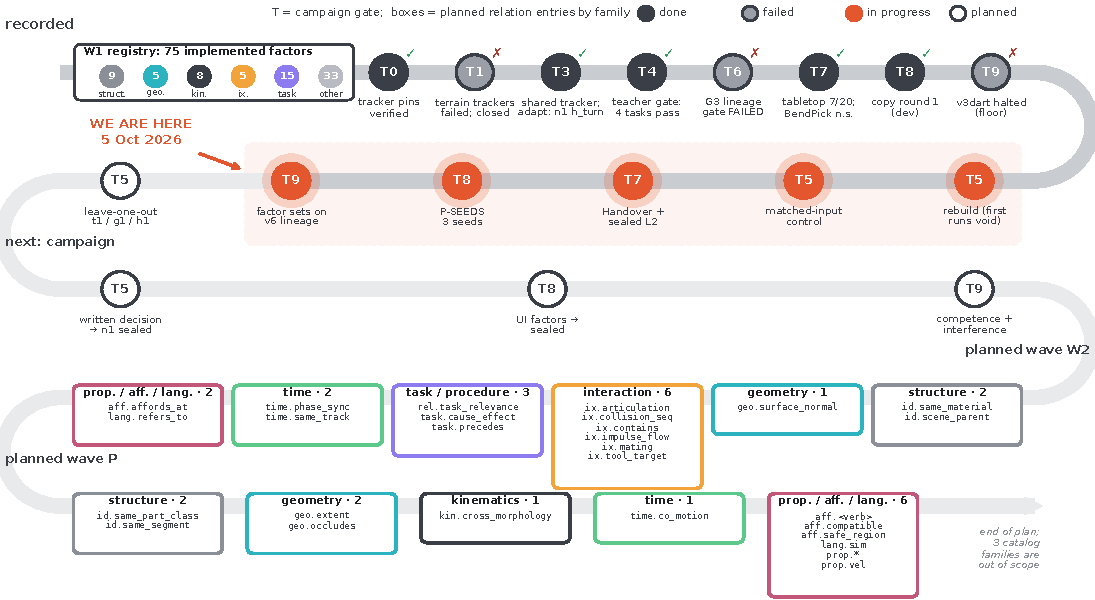
\includegraphics[width=\textwidth]{figures/fig_roadmap.pdf}
\caption{\textbf{Roadmap as of 5 Oct 2026.} The path runs from recorded outcomes (top) to the end of the current plan (bottom). Row 1: the 75 implemented relation factors by family and the recorded gate outcomes, including the failed ones (T1 terrain trackers, T6 G3 lineage gate, T9 v3dart run halted at a floor); T3 adaptation qualified only n1 $\times$ \texttt{h\_turn}. Row 2: the current front (highlighted; the T5 humanoid rebuild after the voided runs, with the matched-input control, T7 HandoverTeleop and the sealed dr-level-2 cells, T8 P-SEEDS, T9 factor sets on the v6 lineage), then the leave-one-out comparison. Row 3: the remaining campaign gates, each ending in sealed or pre-registered readouts (Table~\ref{tab:campaign}). Rows 4--5: every planned entry of Table~\ref{tab:relations-planned}, clustered by its family, wave W2 before wave P; they come after T9 because T9 is the first test of whether factor sets help. Colours follow the families of Fig.~\ref{fig:fig2} (geometry cyan, kinematics graphite, interaction amber, procedure violet; structure, time and property/affordance/language get neutral extra hues). Filled = done, grey with a cross = failed (recorded, not retried), highlighted = in progress, hollow = planned. Generated by \texttt{make\_figures.py roadmap} from the relation registry and catalog.}
\label{fig:roadmap}
\end{figure*}

\paragraph{Humanoid (T0--T5).} Question: with pinned, gated trackers, does the legged relation preset change dev transfer relative to the same recipe without it (\texttt{preset:legged} against \texttt{legged-none}, at least two seeds, matched data and updates)? A tracker is installed only if it passes the D-112 gate, or the labelled D-147 exception (joint margin $\ge-0.06$, peak force $\le4.2$ body weights, cost of transport $\le2.5$, task evaluation $\ge0.9$). One bounded fix per failed gate is allowed. Terrain-scan trackers failed rounds 1 and 2 (T1), so terrain tasks are closed for this campaign; a task with teacher success below 0.8 is held back (T4), which after the re-gate leaves \texttt{h\_walk}, \texttt{h\_turn}, \texttt{h\_reach} and \texttt{h\_squat\_pick}. The test is the dev transfer tables (T5, plus a leave-one-out comparison among t1, g1, h1) followed by a written decision before any sealed cell; no humanoid transfer claim is made until then. The first T5 runs are void (Sec.~\ref{sec:results}) and are being rebuilt under the same pre-registered recipes; the only qualifying sealed cells are n1 $\times$ \texttt{h\_turn}. Because \texttt{legged-none} lacks the terrain scan and limb and foot tokens, a matched-input control (\texttt{legged-tokens}) is pre-registered; ``relation factors help'' needs \texttt{legged} $>$ \texttt{legged-tokens}.

\paragraph{Arm diversity (T6).} H1: a latent route trained on 65 arm $\times$ gripper keys (13 v6 keys, 24 procedural arms and two more menagerie arms, each with two grippers) transfers to new arms better than the v6 13-body lineages, zero-shot and at 5, 20 and 100 target demonstrations, and closes the gap to BC fine-tuning. H2: kinematic static features (\texttt{kinfeat}) help further. Success is $k/100$ per cell with Wilson intervals; three Newcombe contrasts: (a) v8div $-$ v6 latent per primary target, (b) v8div latent $-$ v8div BC fine-tuning at equal budget, (c) kinfeat $-$ no-kinfeat. A contrast counts only if its interval excludes 0; tiers are not pooled; zero-shot is reported apart from adaptation. Gate G3 requires v8div semfix $\ge$ v6 semfix $-0.05$ on the original bodies and a BC expert $\ge0.85$ on the new arms. The BC half passed; the lineage half \textbf{failed} (362/480 vs 425/480, Sec.~\ref{sec:results}), so the track is recorded as \texttt{failed\_hypothesis} and stopped without running any sealed cell; H1 and H2 remain untested.

\paragraph{Packet use in $\Psi_0$ (T7).} Question: does a structured head that reads the packet change closed-loop pick--place relative to direct fine-tuning? The gate requires err\,$R(\bar z)-$err\,$R(E(a))\ge0.05$; a failure ends the node as \texttt{failed\_hypothesis}. It passed on TabletopGraspMP (0.0782) and BendPickMP (0.1483). The closed-loop reading rule, fixed before the BendPickMP and HandoverTeleop results, is per task: structured vs direct with Wilson intervals and paired McNemar; ``structure helps'' only if structured $>$ direct with $p<0.05$, and ``no worse'' is never claimed from overlapping intervals. Tabletop: structured below direct (7/20 vs 19/20). BendPickMP: no difference shown (18/20 vs 15/20, $p{=}0.375$). HandoverTeleop is \emph{in progress}. A sealed test, pre-registered before any level-2 rollout, runs every task $\times$ arm once at domain-randomisation level~2 with the same reading rule; it is \emph{in progress}, and T7 closes for seed~0 after it.

\paragraph{ComputerWorld pointer (T8).} Dev seeds, 50 per task, three training seeds; a difference counts only if it has the same sign in at least two of three paired seeds and exceeds the larger within-arm seed range. P-SEEDS: is the D-142 ordering stable? P-UI: do \texttt{ui.*} factors help (mean gain $\ge4$ points on $\ge2$ tasks, no task losing more than the seed range)? P-COPY: does a copy head fix unseen typing ($\ge10/50$ on both \texttt{open\_type} and \texttt{fill\_form} of \texttt{sealed\_heldout})? P-KEY: does a discrete key code help (dev gain above the seed range)? Sealed sets are evaluated once per arm and seed after the dev table is written. The scripted route cannot copy and is excluded from P-COPY. Round~1 (copy vs free key head, dev) is recorded above; P-SEEDS is \emph{in progress} (interim readings above) and P-UI is planned.

\paragraph{Relation factors (T9).} Question: do the geometry, interaction and task factor sets change arm success relative to the same pipeline without factors? The first run (v3dart, F0-only route) was halted at a floor (0/360 in both arms; uninformative), and the v8div re-plan became moot when G3 failed. The current pre-registration, written before any run, trains the factor sets \{none, geo, ix, task\} $\times$ seeds 1, 2 on the suffix of the v6 semfix lineage, with \texttt{none} on current code as the primary control. A set helps or hurts only if the Newcombe 95\% interval of set $-$ control on the 480 pooled primary cells excludes 0, and the result is valid only if every scheduled factor reaches probe competence $\ge0.5$; per-factor competence by depth and interference are reported alongside. State: \emph{in progress}. Probes and attention maps are diagnostics; causal use is shown by edits and rollouts (Sec.~\ref{sec:results}).

% Table 4 (campaign T0-T9). Fragment: needs booktabs, array, tabularx. Snapshot: campaign/STATUS.md, HANDOFF_*.md and research/decisions.md D-147 addenda through 2026-10-05 ~11:30 PDT.
\providecommand{\st}[1]{{\ttfamily\scriptsize #1}}
\begin{table*}[t]\centering\footnotesize
\setlength{\tabcolsep}{3pt}\renewcommand{\arraystretch}{1.08}
\caption{\textbf{Campaign T0--T9} (D-147; gates from \texttt{research/readiness.md} section B and the D-147 addenda), state as of 5 Oct 2026. States use the repository's progress vocabulary only. A recorded gate outcome is listed when one exists; interim counts of nodes that are still \st{running} are deliberately omitted. ``L'' = body leg length. Teacher checks use the \emph{scripted teacher} (privileged) over a learned tracker.}
\label{tab:campaign}
\begin{tabularx}{\textwidth}{@{}l>{\raggedright\arraybackslash}p{3.2cm}>{\raggedright\arraybackslash}p{4.1cm}>{\raggedright\arraybackslash}p{2.9cm}>{\raggedright\arraybackslash}X@{}}
\toprule
 & Track and run & Pre-registered gate & State & Recorded gate outcome \\
\midrule
T0 & humanoid: pinned trackers and warm starts &
\texttt{t1:contact\_v2} and warm-start checkpoints present with the recorded sha256 &
\st{verified} &
Pins match; its D-112 report reproduces D-114 (no new run). \\
\addlinespace
T1 & humanoid: terrain-scan trackers, \texttt{h\_steps} (t1, g1, h1) and \texttt{h\_gap} (t1, h1), rounds 1 and 2 &
D-112 gate; task eval $\ge$0.9 per height/level; labelled exception only for joint margin, peak force, CoT within caps; one bounded fix per failed gate &
\st{failed\_hypothesis}; \texttt{h\_steps}, \texttt{h\_gap} excluded; terrain closed for D-147 &
Round 1: steps t1 2/20 at 0.10\,L, g1 0/20, h1 10/20 at 0.10--0.15\,L; gap t1 0/20, h1 20/20 but stand falls and force above cap. Round 2: no body passes (t1 steps 0/100). None installable. \\
\addlinespace
T2 & humanoid: wholebody \texttt{*\_ub} gait trackers (t1, g1, h1), \texttt{steps\_ub}, \texttt{h\_carry} teacher check &
Lab gate; teacher check \texttt{h\_carry} $\ge$10/12 both sides, \texttt{h\_steps\_carry} $\ge$8/10, else \st{blocked\_external} &
gait trackers \st{completed}; \texttt{h\_carry} \st{blocked\_external} &
t1, g1, h1 \texttt{ub\_v1} installed under the labelled D-147 exception (joint margin 0.0183 / 0.0191 / 0.0160 against 0.02). \texttt{steps\_ub}: h1 installed, t1 and g1 fail. \texttt{h\_carry}: no plan on g1 / h1. \\
\addlinespace
T3 & humanoid: shared \texttt{morph\_v2\_ub} tracker; sealed-body teacher check; Level-1 adaptation &
Gate on every source body; sealed-body teacher $\ge$16/20 per (body, task), else \st{blocked\_external} &
installed (owner exception); adaptation \st{completed}; n1 $\times$ \texttt{h\_turn} sealed cells pending &
Gate failures carried in the label (op3, adam\_lite, apollo). Sealed-body check: n1 0/40, toddlerbot\_2xc 0/40. After Level-1 adaptation (walk / turn): n1 0/20 / \textbf{16/20 PASS}; 2xc 0/20 / 0/20; 2xm 8/20 / 9/20; berkeley excluded. Only n1 $\times$ \texttt{h\_turn} qualifies. \\
\addlinespace
T4 & humanoid: teacher-quality gate, collection &
Pooled teacher success $\ge$0.8 per task, else held back &
\st{completed} &
Pass: \texttt{h\_walk} 0.95, \texttt{h\_turn} 1.00; re-gate: \texttt{h\_reach}, \texttt{h\_squat\_pick} 60/60. Held back: \texttt{h\_place} 47/60, \texttt{h\_loco\_pick} 33/60; \texttt{h\_carry} \st{blocked\_external}; h1 fails in all three. First collections void ($\sigma{=}0$); re-collected. \\
\addlinespace
T5 & humanoid: \texttt{preset:legged} vs \texttt{legged-none} vs BC, $\ge$2 seeds; leave-one-out t1/g1/h1; matched-input control \texttt{legged-tokens} &
Dev tables, then a \emph{written decision} before any sealed cell; factors help only if legged $>$ legged-tokens &
runs through 4 Oct \textbf{void}; rebuild \st{running} (fair-input caveat on every table) &
Pilot gate check (learned, t1 zero-shot \texttt{h\_turn}): 97/100 [0.915, 0.990], was 0/100; scripted teacher 100/100. Teacher reference g1 \texttt{h\_walk} 78/100. No T5 table yet. \\
\addlinespace
T6 & armdiv: BC 1702, kinfeat BC 1701; G4 signature; v8div lineages $\to$ G3 $\to$ sealed &
BC expert $\ge$0.85 on new training arms; v8div semfix $\ge$ v6 semfix $-0.05$ on original bodies; each sealed cell once &
\st{failed\_hypothesis} (stopped) &
BC gate PASS (117/120 new arms for both). G3 lineage gate \textbf{FAIL}: 362/480 vs 425/480 (threshold 0.835). No sealed cell run. \\
\addlinespace
T7 & $\Psi_0$: labels $\to$ stage A $\to$ packet-use gate $\to$ heads $\to$ closed loop; TabletopGraspMP, BendPickMP, HandoverTeleop &
Gate gap $\ge$ 0.05, else \st{failed\_hypothesis}; closed loop: helps only if structured $>$ direct, McNemar $p<0.05$ &
tabletop, bendpick \st{completed}; handover and sealed L2 \st{running} &
Tabletop: gate PASS 0.0782; structured 7/20 vs direct 19/20 ($p{=}0.0018$); released (upstream) 20/20. BendPick: gate PASS 0.1483; structured 18/20 vs direct 15/20 ($p{=}0.375$, no claim); released (upstream) 20/20. \\
\addlinespace
T8 & pointer v2: collection $\to$ copy / key heads $\to$ seeds $\to$ UI factors, dev tables &
P-KEY, P-COPY, P-SEEDS, P-UI rules (Sec.~\ref{sec:campaign}); sealed only after a written decision &
collection, copy round \st{completed}; seeds \st{running}; UI \st{planned} &
Collection 4$\times$6{,}000 teacher episodes. Oracle packets $\to$ scripted System~0: 50/50 per task (privileged reference). Copy head worse than free head on drag (dev). Seeds: no decision until all three seeds land. \\
\addlinespace
T9 & relation factors: \{none, geo, ix, task\} $\times$ seeds 1, 2 on the v6 semfix lineage &
Newcombe 95\% of set $-$ none excludes 0; valid only if every factor's competence $\ge0.5$ &
v3dart run halted (\st{failed\_hypothesis}, floor); v8div moot; v6 run \st{running} &
v3dart: 0/360 vs 0/360, uninformative. v6: training in progress, no evaluation yet. \\
\bottomrule
\end{tabularx}
\end{table*}


% Limitations. Fragment.
\section{Limitations}\label{sec:limitations}
The evidence is narrow. (i) \emph{No cross-body transfer claim.} Zero-shot transfer to new arms is 0/200 for every method, the latent route has not beaten BC on any new body, the arm-diversity lineage gate failed before any sealed new-arm cell, and no sealed humanoid cell has run (after adaptation only n1 $\times$ \texttt{h\_turn} qualifies; its cells are pending). (ii) \emph{Seeds.} Most ComputerWorld numbers are one training seed (D-142); the legged result has three seeds per body (D-124), with exact seed-ordering $p{=}0.05$. Intervals cover evaluation episodes, not training-seed variance. (iii) \emph{Post-hoc analysis.} The joint-adaptation method of D-136 was added after the sealed results of D-135 on the same scenes; it is labelled and not a pre-registered test. (iv) \emph{Partial edits.} Packet edits move behaviour part of the way (the probe reads the edit in 8--10 of 25 cases) and are demonstrated on calculator and form tasks only. (v) \emph{Unseen strings.} With the v1 packet all learned pointer methods fail on unseen typing and form text (0/100, sealed). The v2 key code types held-out-bucket strings on development seeds, but no sealed v2 evaluation exists yet. (vi) \emph{Pretrained humanoid.} After the integration fix the structured head reaches 7/20 against 19/20 for direct fine-tuning on one task and 18/20 against 15/20 (not significant) on a second, one seed each, $n{=}20$; HandoverTeleop and the sealed level-2 test are in progress. (vii) \emph{Humanoid trackers.} Terrain trackers failed their gates, so terrain tasks are out of this campaign; the installed gait and shared trackers are labelled exceptions to the D-112 gate. The first humanoid transfer runs were voided by two pipeline bugs (gait-clock offset, DART noise never applied), found only because learned cells scored 0/100 against a 100/100 teacher; the rebuild has passed one pilot gate check. The legged vs legged-none comparison mixes relation factors with extra inputs until the matched-input control lands. (viii) \emph{Simulation.} All results are simulated, with scripted or privileged teachers; sim-truth labels train probes and are not deployable inputs. No physical robot was commanded. (ix) \emph{Snapshot.} This is a living report of an ongoing campaign (snapshot 5 Oct 2026); running nodes may finish with results that are not shown here.


\begingroup\small\setlength{\parskip}{0pt}\setlength{\itemsep}{0pt}
\begin{thebibliography}{9}\setlength{\itemsep}{0pt}\setlength{\parsep}{0pt}
\bibitem{psi0} S.~Wei \emph{et al.} $\Psi_0$: An open foundation model towards universal humanoid loco-manipulation. arXiv:2603.12263, 2026.
\bibitem{pape} C.\,K.~{\O}hrstr{\o}m \emph{et al.} Parabolic position encoding: vision-centric, principled, extrapolatable, general (PaPE). arXiv:2602.01418, 2026.
\bibitem{rectflow} X.~Liu, C.~Gong, Q.~Liu. Flow straight and fast: learning to generate and transfer data with rectified flow. arXiv:2209.03003, 2022.
\bibitem{fm} Y.~Lipman \emph{et al.} Flow matching for generative modeling. arXiv:2210.02747, 2022.
\bibitem{battaglia} P.\,W.~Battaglia \emph{et al.} Relational inductive biases, deep learning, and graph networks. arXiv:1806.01261, 2018.
\bibitem{mujoco} E.~Todorov, T.~Erez, Y.~Tassa. MuJoCo: a physics engine for model-based control. IROS, 2012.
\bibitem{menagerie} Google DeepMind. MuJoCo Menagerie: a collection of high-quality simulation models for MuJoCo. \texttt{github.com/google-deepmind/mujoco\_menagerie}, 2022.
\end{thebibliography}\endgroup

\appendix
\section{Relation tables (generated)}\label{app:relations}
Both tables are written by \code{make\_figures.py table\_relations} from the live registries and the candidate catalog; nothing about an implemented factor is typed by hand.
\relfull
Fig.~\ref{fig:tiles} draws every row of Table~\ref{tab:relations} as one tile: the factor's term for one query token on a real simulator or environment state, computed by the same operator and label code the model uses, with hand-set coefficients where the model learns them. It extends Fig.~\ref{fig:fig2} from eight panels to all implemented factors and, like it, shows no trained attention. Badges separate public (given) terms from probe-sourced ones, whose tiles show the simulator-truth label that trains the probe (training-only); the deployed term is the estimated-probe value. Under each tile its caption gives what the term encodes on the shown state, the operator and form with the hand-set coefficients, the term's source and its equation. Tiles marked illustrative are not fully computable from shipped code or data; their caption gives the reason.
\tilegrid
\relplanned

\section{Embodiment count (generated)}\label{app:embodiments}
Table~\ref{tab:embodiments} is written by \code{make\_figures.py embodiments}, which reads the teacher-validation records, the arm admission screens, the dual-arm teacher validation, the legged body catalog, the tracker training metadata (host store and the host copy of the peer archive) and the frozen splits, and keeps the per-class key lists in \code{figures/embodiments.json}.
\embtable

\end{document}
